\documentclass[conference]{IEEEtran}
\IEEEoverridecommandlockouts
% The preceding line is only needed to identify funding in the first footnote. If that is unneeded, please comment it out.
\usepackage{cite}
\usepackage[ngerman]{babel}
\usepackage[utf8]{inputenc}
\usepackage{amsmath,amssymb,amsfonts}
\usepackage{algorithmic}
\usepackage{graphicx}
\usepackage{textcomp}
\usepackage{xcolor}
\usepackage{listings}
\usepackage{bbold}
\usepackage{subfigure}


\definecolor{pblue}{rgb}{0.13,0.13,1}
\definecolor{pgreen}{rgb}{0,0.5,0}
\definecolor{pred}{rgb}{0.9,0,0}
\definecolor{pgrey}{rgb}{0.46,0.45,0.48}
\lstset{language=Python,
	showspaces=false,
	showtabs=false,
	breaklines=true,
	tabsize=2,
	showstringspaces=false,
	breakatwhitespace=true,
	commentstyle=\color{pgreen},
	keywordstyle=\color{pblue},
	stringstyle=\color{pred},
	basicstyle=\ttfamily
}


\usepackage{url}
\def\BibTeX{{\rm B\kern-.05em{\sc i\kern-.025em b}\kern-.08em
		T\kern-.1667em\lower.7ex\hbox{E}\kern-.125emX}}
\begin{document}
	
	\title{Videoanalyse und Objekttracking}
	
	\author{\IEEEauthorblockN{1\textsuperscript{st} Bartolovic Eduard}
		\IEEEauthorblockA{\textit{Hochschule München} \\
			München, Deutschland \\
			eduard.bartolovic0@hm.edu}
		\and
		\IEEEauthorblockN{2\textsuperscript{nd} Thomas Willeit}
		\IEEEauthorblockA{\textit{Hochschule München} \\
			München, Deutschland \\
			twilleit@hm.edu@hm.edu}
		\and
		\IEEEauthorblockN{3\textsuperscript{rd} Schäfer Julia}
		\IEEEauthorblockA{\textit{Hochschule München} \\
			München, Deutschland \\
			j.schaefer0@hm.edu}
	}
	
	
	\maketitle
	
	\begin{abstract}
		In Zeiten, in denen Neuronale Netze immer mehr Bedeutung erlangen ist es wichtig weiterhin die klassischen Algorithmen zu berücksichtigen, da diese oftmals ähnlich gute Ergebnisse erzielen. Im Rahmen der Veranstaltung Videoanalyse und Objekttracking wurden daher zwei mögliche Umsetzung für Objekt-Detektion und zwei für Objekt-Tracking näher betrachtet und implementiert. Jeweils eine der Umsetzung je Themenbereich arbeitet auf Basis von Neuronalen Netzen. Anschließend wurden für beide Varianten ein Objektzähler implementiert der die erkannten Objekte zählt. Ein wichtiger Bereich sind ebenfalls Fehler und Probleme der Algorithmen, welche anhand von aufgezeichneten Daten erläutert werden. Zuletzt wird ein Vergleich von klassischen Algorithmen mit Algorithmen auf Basis von Neuronalen Netzen gegeben.
	\end{abstract}
	
	
	\section{Videomaterial}
	Für dieses Projekt wurden mehrere Aufnahmen aufgenommen. Ziel war es keine zu chaotischen, aber auch nicht zu einfache Aufnahmen zu erstellen. Auch sollten verschiedene Szenarien abgebildet werden. Es wurden drei Aufnahmen angefertigt.\\
	\textbf{Verkehrsaufnahmen am Brudermühltunnel am Mittleren Ring:}\\
	Dieser Teil des Mittleren Rings ist sehr verkehrsreich und Autobahnähnlich ausgebaut. Es gibt mehrere Fahrspuren. Alle Fahrzeuge fahren im Sichtfeld in eine Richtung. Es sind ein paar Laternen und Bäume in der Aufnahme die die Sicht etwas beeinträchtigen. Es sind nur Pkw im Datensatz enthalten. Teilweise missachten Fahrzeuge den Sicherheitsabstand und fahren sehr nah aufeinander auf. Dies erschwert die Detektion. Das Video wurde in 60 Bilder pro Sekunde aufgezeichnet und hat eine Bildauflösung $3840$ × $2160$. Es wurde kein Stativ verwendet, sondern nur die interne Stabilisierung des Smartphones genutzt.
	\begin{figure}[!h]
		\begin{center}
			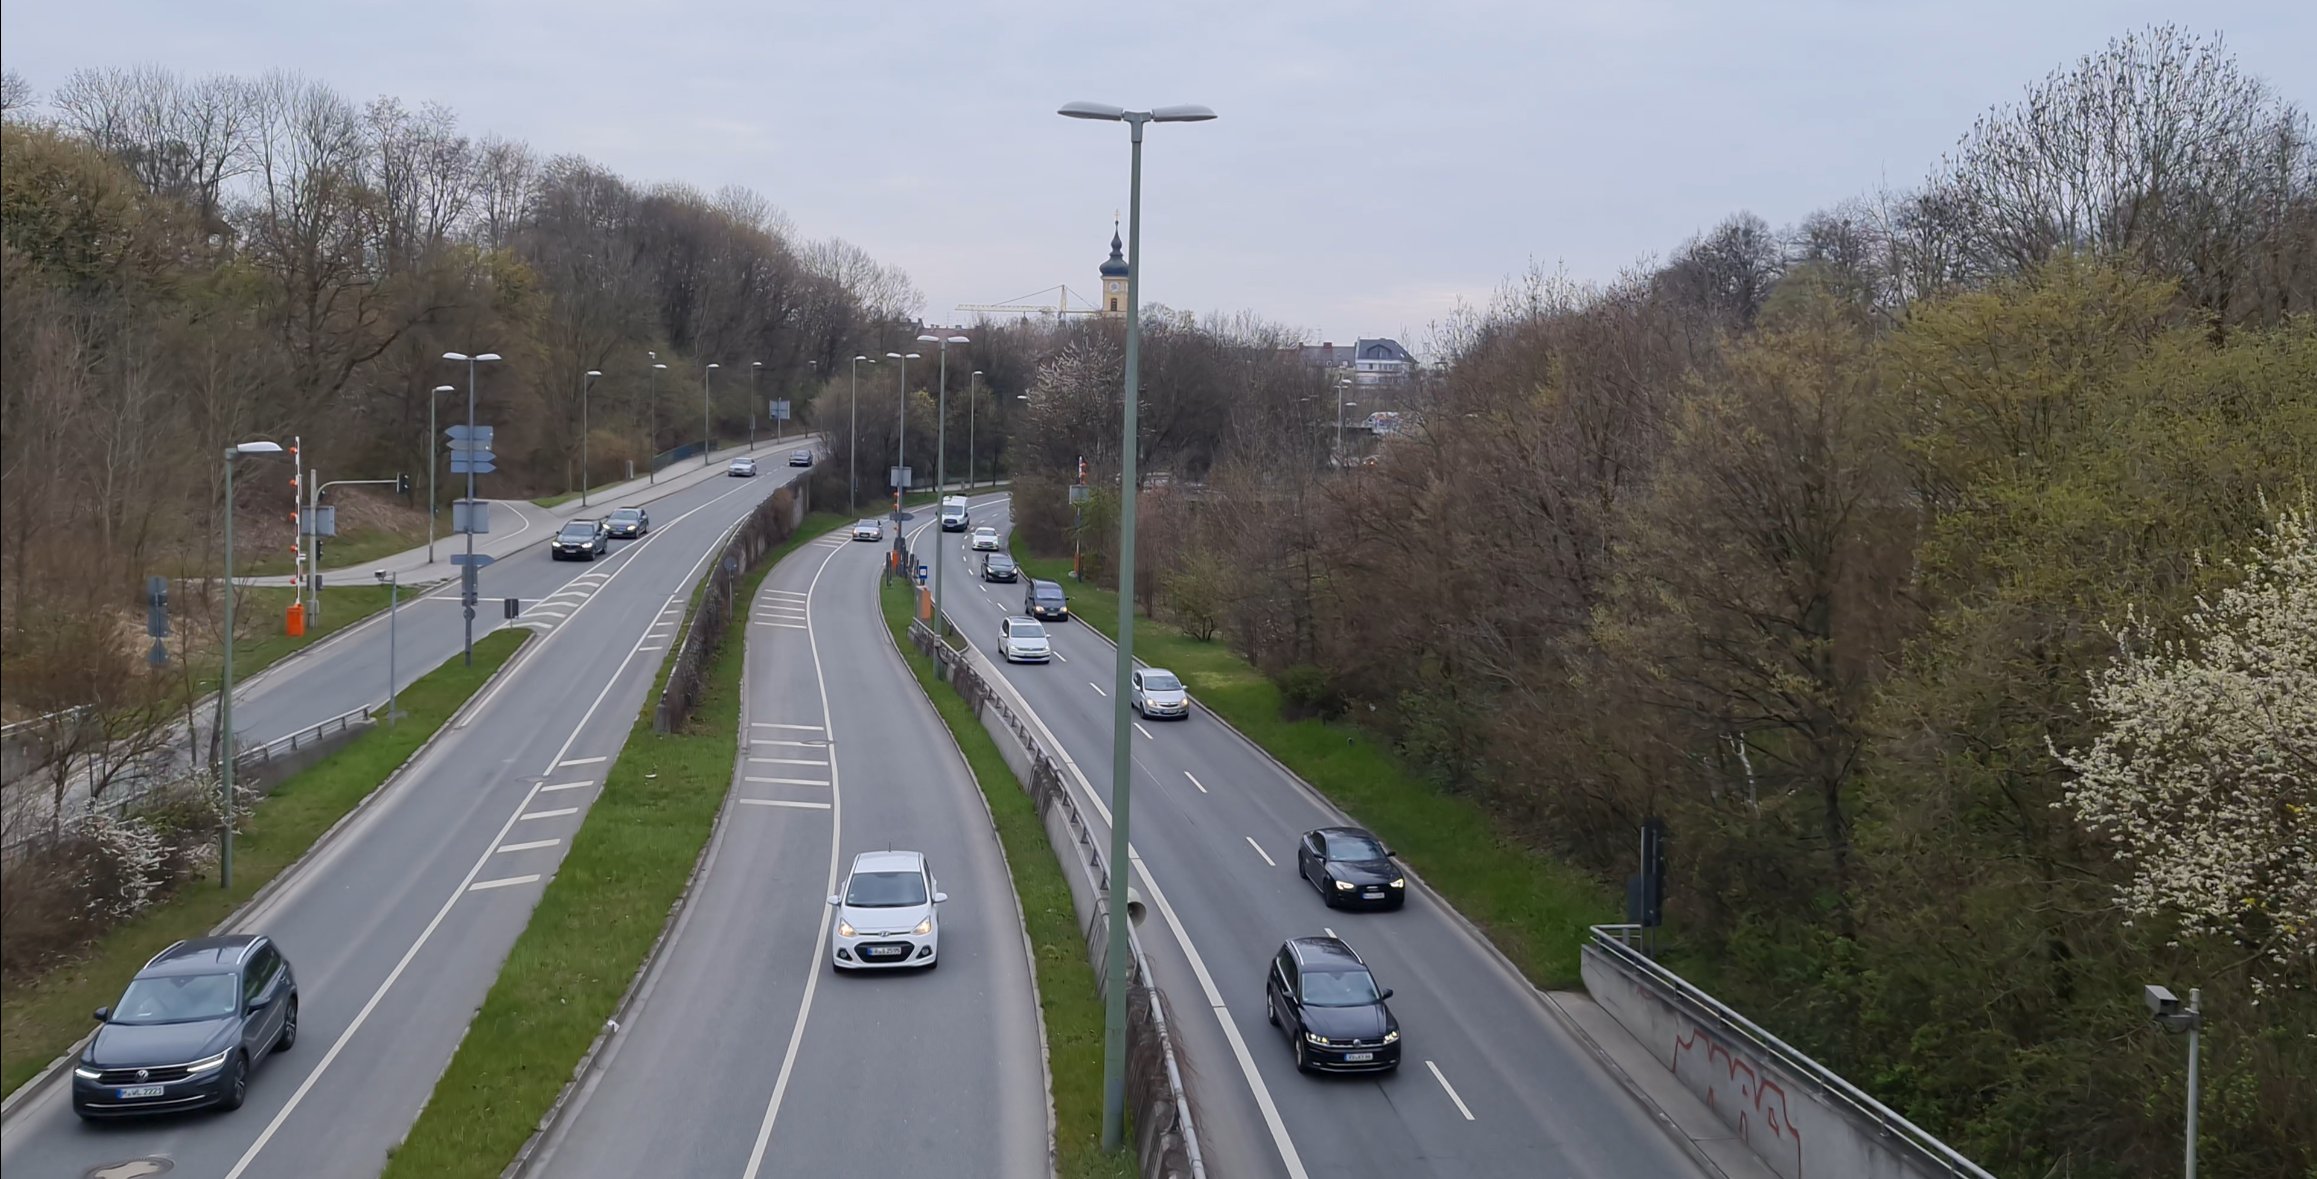
\includegraphics[width=8cm]{Media/BrudermuhlRaw.png}
			\caption{Verkehrsaufnahmen am Brudermühltunnel}
			\label{BrudermuhlRaw}
		\end{center}
	\end{figure}\\
	\textbf{Verkehrsaufnahmen am Candidtunnel:}\\
	Eine stark befahrene Straße mit einer Vielzahl von Verkehrsteilnehmern. Es herrscht Zweirichtungsverkehr mit insgesamt sechs Fahrspuren. In eine Richtung stehen die Fahrzeuge in einem Stau. Durch Regen spiegeln viele Oberflächen. Die Bäume bewegen sich aufgrund von stärkeren Wind und verdecken einen Teil der Fahrbahn. Diese Aufnahme ist die Anspruchsvollste. In diesem Video sind neben Pkw auch Busse enthalten. Das Video hat 60 Bilder pro Sekunde und eine Bildauflösung von $3840$ × $2160$. Es wurde kein Stativ verwendet sondern nur die interne Stabilisierung des Smartphones genutzt.
	\begin{figure}[!h]
		\begin{center}
			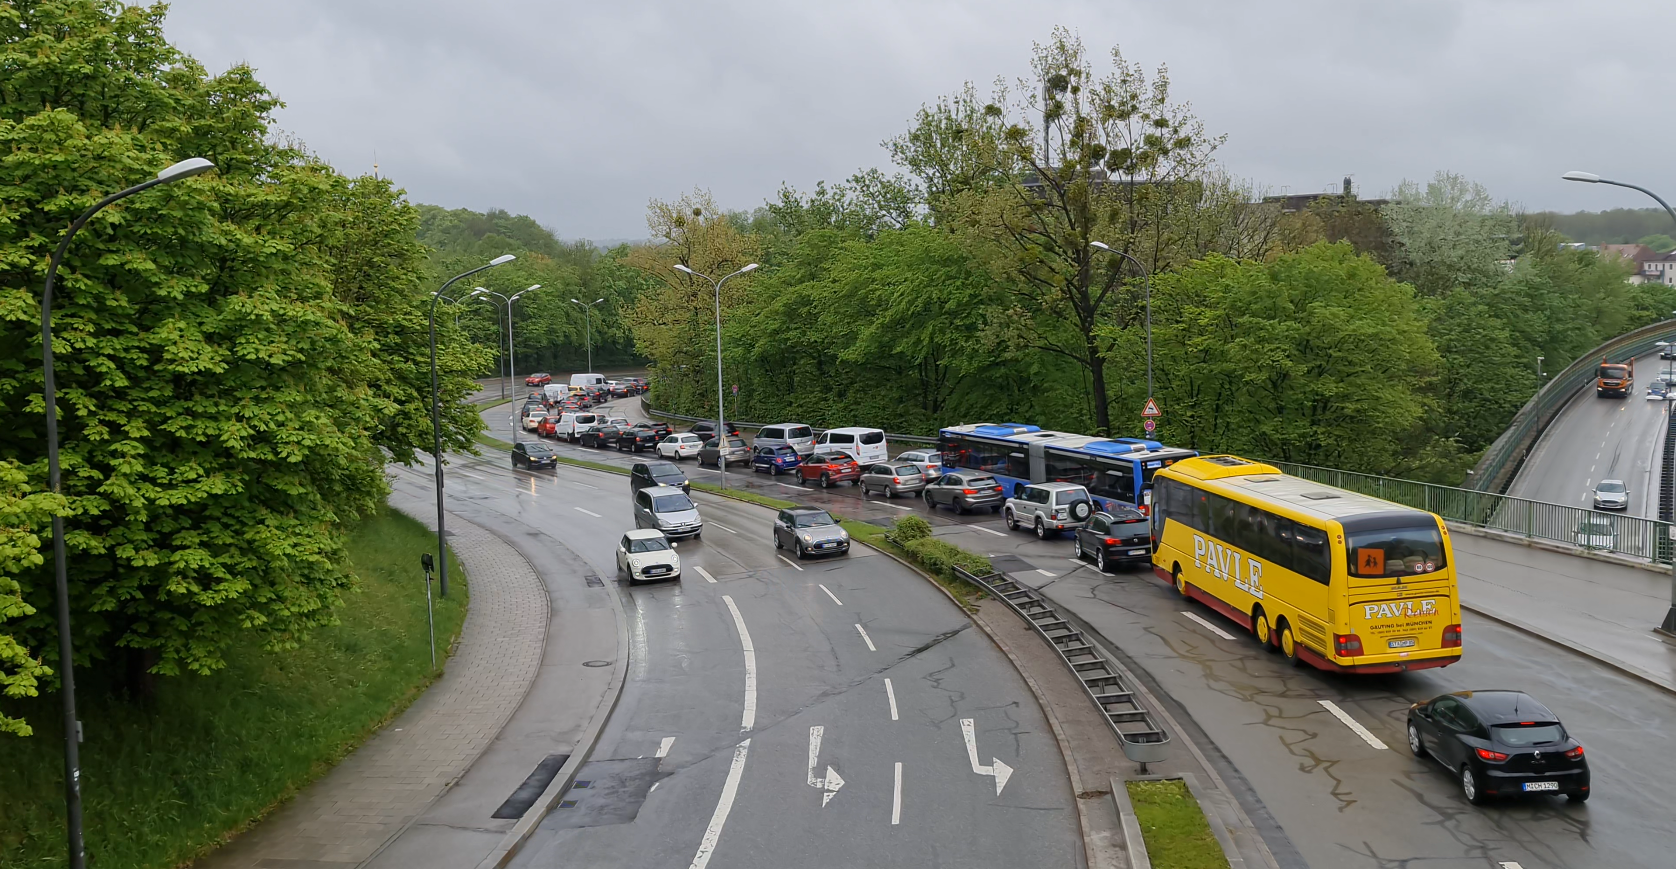
\includegraphics[width=8cm]{Media/CandidRaw.png}
			\caption{Verkehrsaufnahmen am Candidtunnel}
			\label{CandidtunnelRaw}
		\end{center}
	\end{figure}\\
	\textbf{Zugaufnahmen an der Donnersbergerbrücke:}\\
	Eine Aufnahme einer der am stärksten befahren Bahnstrecken Europas\cite{z1}. Hier existiert viel Zugverkehr auf mehreren Gleisen mit unterschiedlichen Zugtypen. Beobachtet werden die vier Gleise der zwei Bahnsteige des S-Bahnhalts Donnersbergerbrücke. Ein Hindernis sind die Masten, Signale, Bäume und das Bahnsteigdach welche einen guten Blick auf die Züge erschweren. In dieser Aufnahme sind Züge und Fußgänger enthalten. Der Fokus liegt aber auf den Zügen. Das Video hat 30 Bilder pro Sekunde und hat eine Bildauflösung $1920$ × $1080$. Es wurde ein Stativ verwendet.\\
	\begin{figure}[!h]
		\begin{center}
			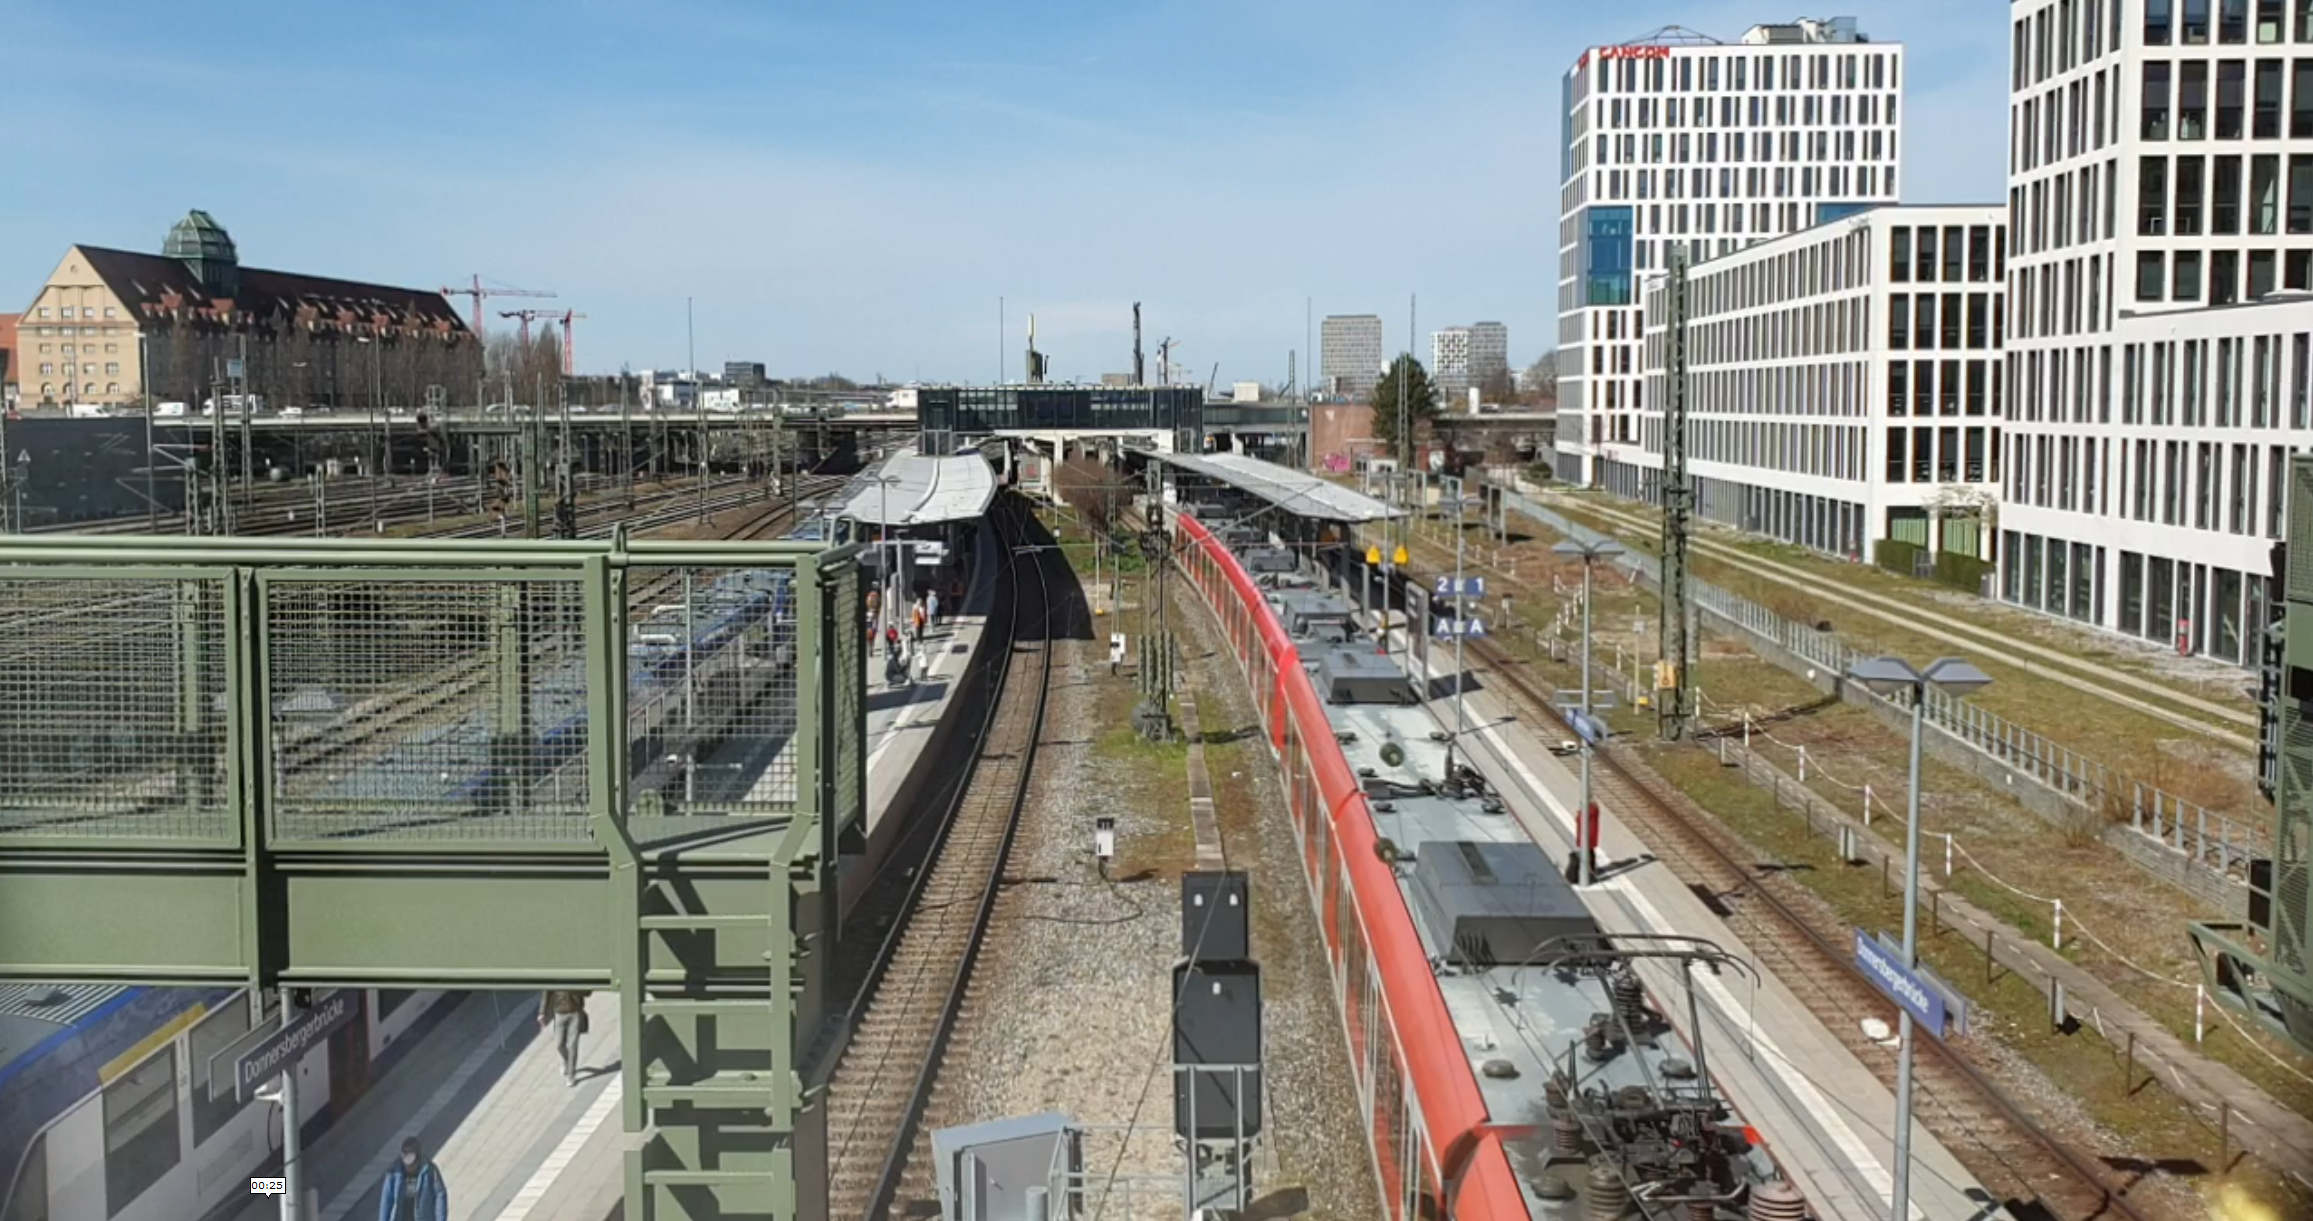
\includegraphics[width=8cm]{Media/DonnersbergerRaw.png}
			\caption{Zugaufnahmen an der Donnersbergerbrücke}
			\label{DonnersbergerRaw}
		\end{center}
	\end{figure}
	
	\begin{figure*}[!h]
		\begin{center}
			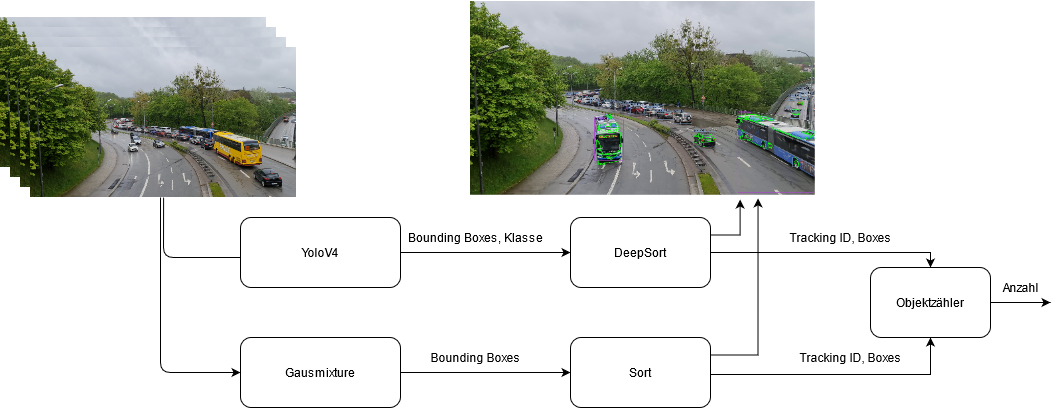
\includegraphics[width=16cm]{Media/KonzeptVAOT.png}
			\caption{Konzept für das Projekt mit zwei Pipelines.}
			\label{Konzept}
		\end{center}
	\end{figure*}
	
	\section{Konzept}
	Ziel des Projektes ist es klassische Verfahren mit neueren DeepLearning Methoden zu vergleichen.
	Dafür ist für beide Arten eine Pipeline geschaffen worden.\\
	Für die klassischen Methoden wurde für die Objekterkennung das Gausmixture Verfahren verwendet und für das Tracking der SORT Algorithmus. Für die DeepLearning Verfahren wurde für die Objekterkennung ein Neuronales Netz und für das Tracking wurde Deepsort verwendet.\\
	Mit einem Objektzähler können am Ende der beiden Pipelines die Objekte gezählt oder mit einer Zustandserkennung die Bewegungen und Stillstand erfasst werden. Die Abbildung \ref{Konzept} visualisiert das Konzept.\\
	Bilder werden mittels der OpenCV Bibliotheksmethoden Frame für Frame aus einem Video ausgelesen.
	Bevor mit der Erkennung von Objekten begonnen werden kann, werden die Videoaufnahmen so erstellt, angepasst und eingeschränkt, dass bessere Ergebnisse bei der Erkennung erzielt werden können.
	\section{Preprocessing}
	Es ist möglich Bilder vor der weiteren Verarbeitung noch beliebig zuzuschneiden, um nur relevant Bereiche zu betrachten. Dies hat den Vorteil, dass die Performance steigt und auch die Genauigkeit mancher Algorithmen zunimmt. Diese Bilder werden anschließend in die Pipeline gelegt.\\
	Bevor das Zuschneiden beginnt, kann während und nach der Videoaufnahme, das Video stabilisiert werden.
	\subsection{Videostabilisierung}
	Es gibt folgende Ansätze zur Videostabilisierung:\\
	\textbf{Mechanische Videostabilisierung:}\\
	Im ersten Ansatz versucht man unerwünschte Bewegungen im Video, die durch das Wackeln der Hand entstehen, durch ein Kamerastativ oder ein Gimbal, welches mit Hilfe von Sensoren Bewegungen ausgleicht, zu vermeiden. Diese Art der Stabilisierung findet vor bzw. während der Aufnahme statt.
	In unserer Aufnahme der Donnersbergerbrücke wurde ein Stativ verwendet.\\
	\textbf{Optische Videostabilisierung:}\\
	Die zweite Vorgehensweise bewegt anders als im vorherigen Absatz genannt nicht die gesamte Kamera, sondern nur Teile im Objektiv oder beim Bildsensor. Es wird also entweder der Bildkreis über dem Bildsensor oder der Bildsensor unter dem Bildkreis verschoben. Beschleunigungssensoren erkennen hier die Bewegung der Kamera und passen dementsprechend die optischen Elemente an, damit das Bild stabilisiert wird. Das Ganze findet während der Aufnahme statt.\\
	\textbf{Digitale Videostabilisierung:}\\
	Der letzte Ansatz erfolgt nach der Aufnahme über Software und es ist keine zusätzliche Hardware nötig. Mit Hilfe von Algorithmen werden die Unterschiede zwischen zwei hintereinander folgenden Frames herausgefunden, unerwünschte Bewegungen entfernt und Anschluss zu einem stabilisierten Video zusammengefügt. Im Folgenden soll diese Art der Stabilisierung vorgestellt werden.
	Dabei wird nicht genauer auf die mathematischen Hintergründe eingegangen, sondern nur die Vorgehensweise beschrieben und auf die Algorithmen dahinter verwiesen \cite{stab}.\\
	\textbf{Videostabilisierung - Implementierung:}
	\begin{enumerate}
		\item Im ersten Schritt werden die Frames eingelesen und in ein Grauwertbild umgewandelt.
		
		\item Anschließend wird die Bewegung zwischen dem aktuellen und dem vorherigen Frame bestimmt. Theoretisch würden 2 Punkte zur Bestimmung reichen, allerdings sollten für eine stabile Schätzung deutlich mehr Punkte verwendet werden.
		Bildregionen mit besonders vielen Ecken eignen sich hier äußerst gut, weshalb mithilfe von goodFeaturesToTrack() von OpenCV die gewünschten Features detektiert werden.
		Diese Funktion besteht aus einer Modifikation des Harris-Corner-Detectors durch Shi-Tomasi.
		\begin{figure}[!h]
			\begin{center}
				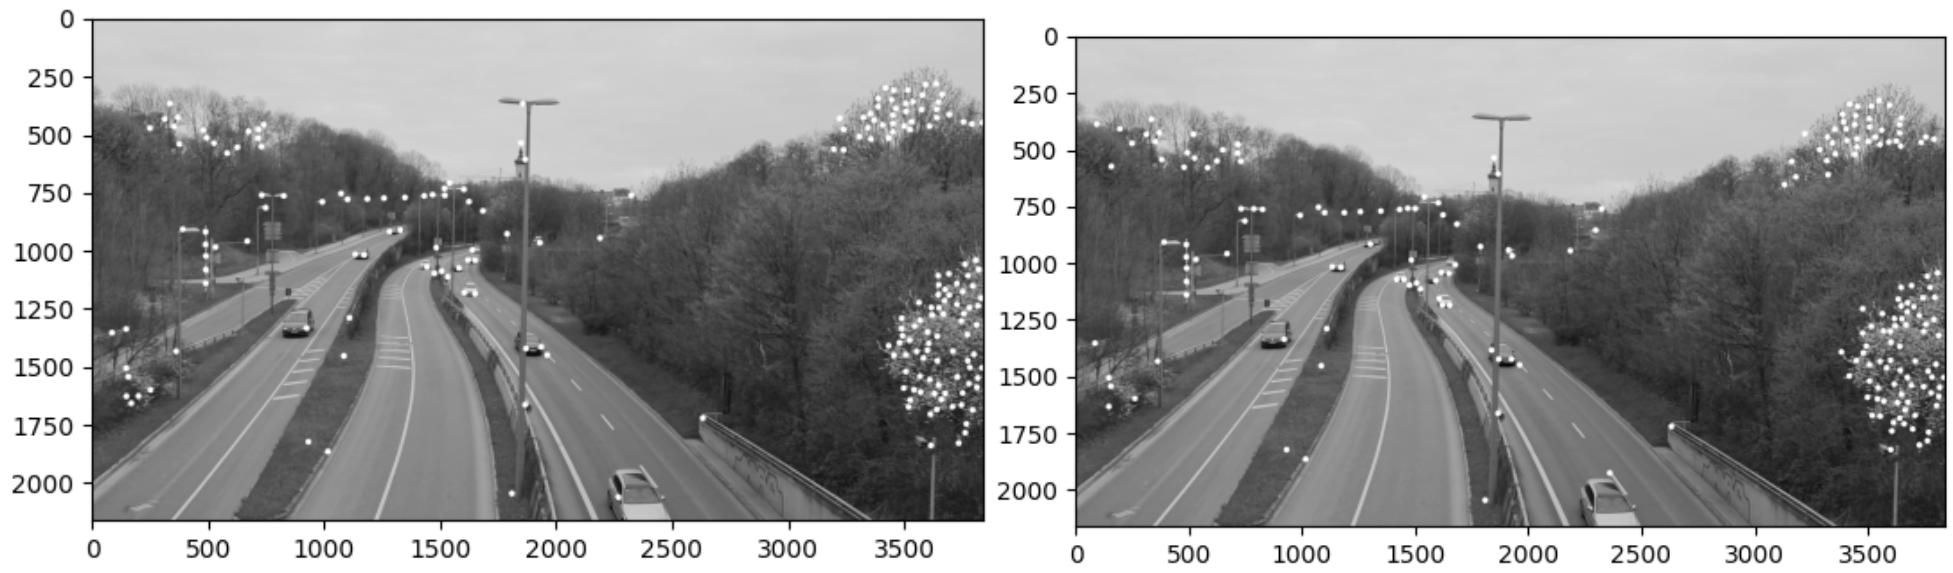
\includegraphics[width=8cm]{Media/VideoStab.png}
				\caption{Shi-Tomasi Corner Detector: Good Features to Track}
				\label{VS1}
			\end{center}
		\end{figure}
		
		\item Danach kann mit der Lucas-Kanade Methode der Optical Flow bestimmt werden. Wie in der Abbildung \ref{VS2} zu sehen ist werden sowohl die Bewegungen der Fahrzeuge als auch Bewegungen in den Bäumen oder den Straßenlaternen im Hintergrund eingezeichnet. Diese sind geringer als die Bewegung der Fahrzeuge und entstehen durch das Wackeln der Hand beim Filmen. Sie könnten allerdings auch durch Wind verursacht werden, wodurch es zu einem Fehler bei der Stabilisierung kommen könnte.
		
		\begin{figure}[!h]
			\begin{center}
				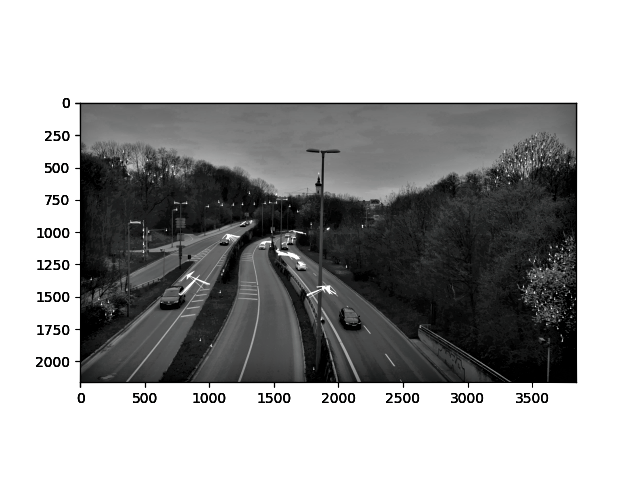
\includegraphics[width=8cm]{Media/VideoStab2.png}
				\caption{Lucas-Kanade Optical Flow: Bewegungen im Bild}
				\label{VS2}
			\end{center}
		\end{figure}
		
		\item Da nun die Features im aktuellem und dem Frame davor bekannt sind, lässt sich daraus die affine Transformation zwischen den beiden Bildern mit estimateRigidTransform() berechnen. Daraus wird dann die Translation in x, y-Richtung und die Rotation herausgeholt und für den späteren glatteren Übergang abgespeichert.
		
		\item Nach Durchlaufen aller Frames wird mit np.cumsum die kumulierte Summe aller gespeicherten Transformationen und somit die Trajektorie erstellt.
		
		\item Nun liegen 3 Kurven vor, die die Veränderung der Bewegung (x, y, Winkel) über die Zeit darstellen. Diese Kurven werden nun mit dem Bewegten Mittelwert geglättet. Um den Bewegten Mittelwert zu verstehen, betrachten wir das folgende Beispiel: 
		Eine Kurve ist in einem Array c gespeichert und die Filtergröße ist 5. Möchten wir nun das k-te Element glätten ergibt sich die folgende Berechnung:
		\[ f[k] = \frac{c[k-2]+c[k-1]+c[k]+c[k+1]+c[k+2]}{5} \]
		
		\item Im letzten Schritt wird der Unterschied zwischen der originalen und der geglätteten Trajektorie berechnet und auf die ursprüngliche Transformation addiert, wodurch man eine geglättete Transformation erhält. Diese wird nun auf die Frames angewandt. Um Artefakte zu vermeiden, werden die Bilder um den Bildmittelpunkt minimal skaliert, dadurch können schwarze „Flecken“ an den Bildrändern vermieden werden, solange die Kamerabewegungen nicht zu extrem sind \cite{s1}\cite{s2}\cite{s3}\cite{s4}.
		
	\end{enumerate}
	\textbf{Videostabilisierung – Ergebnis:}\\
	In der Abbildung \ref{VS3} sieht man links die Detektion auf dem Originalvideo und rechts die Detektion auf dem stabilisierten Video. Während die Fahrzeugdetektion fast identisch ist, fällt auf, dass die Bewegungen in den Bäumen und der restlichen Umgebung deutlich geringer sind. Zwar konnten nicht alle unerwünschten Bewegungen entfernt werden, aber es konnte eine sichtbare Verbesserung erzielt werden.
	\begin{figure*}[!h]
		\begin{center}
			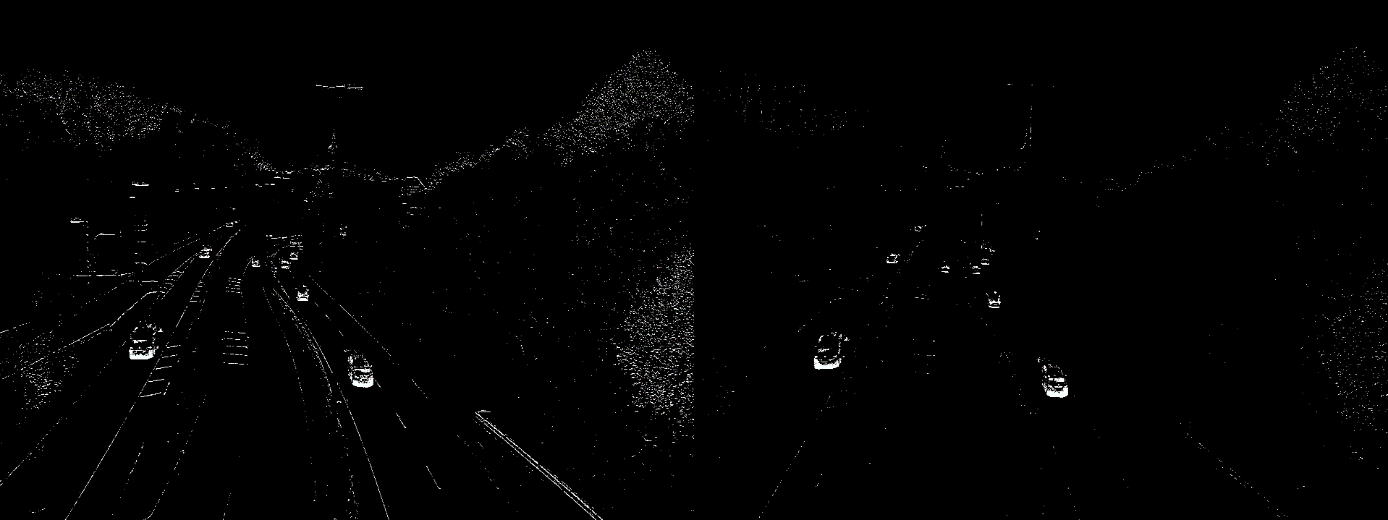
\includegraphics[width=16cm]{Media/VideoStab3E.png}
			\caption{Links: ohne Videostabilisierung; Rechts: mit Videostabilisierung}
			\label{VS3}
		\end{center}
	\end{figure*}\\
	\textbf{Videostabilisierung – Alternativer Ansatz:}\\
	Die restlichen weißen Bildpunkt werden durch Anwendung einer Erosion entfernt und die übrig gebliebenen Fahrzeuge wieder mit einer Dilatation deutlich gemacht.
	Wie in der folgenden Bilderfolge zu sehen ist, verschwinden durch die Erosion die unerwünschten Bewegungen, die nicht durch die Videostabilisierung entfernt werden konnten. Die nun kaum sichtbaren Flächen der Fahrzeuge werden mit der Dilatation so weit vergrößert, dass diese wieder gut zu detektieren sind \cite{ed}. Die Schritte werden in den Grafiken \ref{MOGPart1} bis \ref{MOGPart4} gezeigt.\\
	\begin{figure}
		\begin{subfigure}{}
			\centering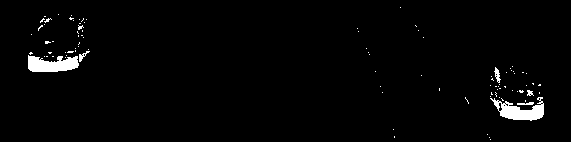
\includegraphics[width=7cm]{Media/MOG1.png}
			\caption{Mixture of Gaussian}
			\label{MOGPart1}
		\end{subfigure}
		\vspace{5pt}
		\begin{subfigure}{}
			\centering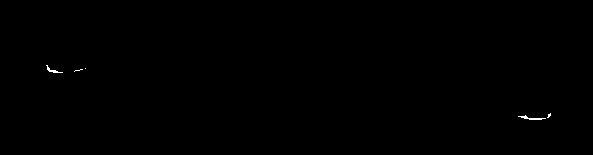
\includegraphics[width=7cm]{Media/MOG2.png}
			\caption{Ergebnis der Erosion auf Mixture of Gaussian}
		\end{subfigure}
		\vspace{5pt}
		\begin{subfigure}{}
			\centering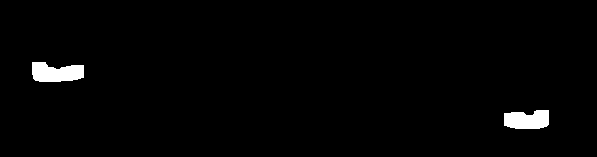
\includegraphics[width=7cm]{Media/MOG3.png}
			\caption{Ergebnis der Dilatation auf Erosion}
		\end{subfigure}
		\vspace{5pt}
		\begin{subfigure}{}
			\centering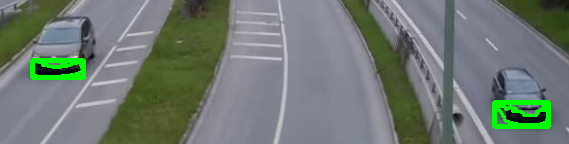
\includegraphics[width=7cm]{Media/MOG4.png}
			\caption{Objekterkennung}
			\label{MOGPart4}
		\end{subfigure}	
	\end{figure}
	
	
	\section{Objekterkennung: MOG-Mixture of Gaussian}
	Ziel des Mixture of Gaussian Algorithmus ist, den unbewegten Hintergrund zu erkennen und diesen vom Bild zu subtrahieren. Das heißt alle Pixel, die zum Hintergrund gehören, werden schwarz und alle anderen weiß dargestellt. Anschließend können mit cv2.findContours() zusammenhängende weiße Pixel zu Objekten hinzugefügt werden. Wenn die Fläche der Pixel einen definierten Threshold überschreitet, wird um diese eine Bounding Box eingezeichnet.\\
	\textbf{Funktionsweise MOG}\\
	Im ersten Schritt wird der Funktion eine Anzahl an Frames zum „Lernen“ zugeteilt. Aus diesen wird der unbewegte Hintergrund bestimmt, welcher später subtrahiert wird, sodass nur die bewegten Objekte übrigbleiben.
	Der Algorithmus modelliert für jeden Pixel den Hintergrund mit unterschiedlich gewichteten Gauss-Funktionen $\eta$.  Diese K-Funktionen enthalten eine Gewichtung $(\omega_i,t)$, den durchschnittlichen Intensitätswert $(\mu_i,t)$ und die Standardabweichung $(\sigma_i,t)$ für den i-ten Gaussian zum Zeitpunkt t.
	\[ \sum_{i-1}^{K} \omega_i,t * \eta(u; \mu_i,\sigma_i)  \]
	Mit jedem neuen Pixel (z.B. Kamerabewegung oder Fahrzeugbewegung) werden die Gauss-Funktionen frameweise geupdatet. Dabei wird die Pixelhistorie und der neue Pixelwert berücksichtigt. Falls nun zu einem neuen Pixel keiner der Gauss-Funktionen innerhalb eines Thresholds passt, wird der Pixel als Vordergrund deklariert, ansonsten als Hintergrund. Diese adaptive Hintergrundsubtraktion mit MOG wird in Abbildung \ref{mogKonzept} gezeigt.\\
	\begin{figure}[!h]
		\begin{center}
			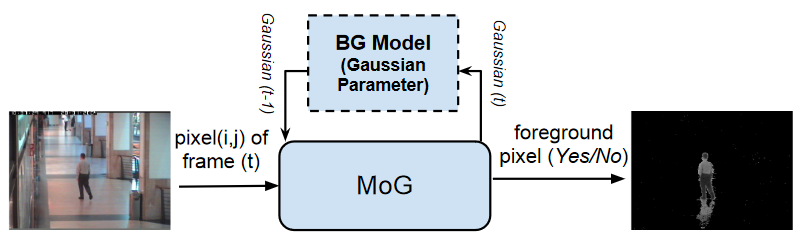
\includegraphics[width=7cm]{Media/MOGKONZEPt.png}
			\caption{Adaptive Hintergrundsubtraktion mit MOG \cite{mog1}}
			\label{mogKonzept}
		\end{center}
	\end{figure}
	Vereinfacht beschrieben misst der Algorithmus in den Lernbildern die Zeit, in welcher ein Pixel den gleichen Intensitätswert hat und bestimmt so den Hintergrund. Ändert sich nun dieser Wert, wird an dem Pixel eine Bewegung erkannt, dieser als Vordergrund bestimmt und die Parameter geupdatet \cite{m1}\cite{m2}\cite{m3}\cite{m4}.\\
	\\
	\textbf{Probleme MOG}\\
	Eine Schwierigkeit bei der Objekterkennung ist, dass die Bewegungen hauptsächlich bei großen Intensitätsunterschieden wie der Wechsel von Straße zu Fahrzeuganfang und von Fahrzeugende zur Straße, erkannt werden. Große Flächen wie die Motorhaube, Windschutzscheibe und die Dachfläche werden nicht erkannt, da diese so lange einen Pixel mit einem sehr ähnlichen Intensitätswert „bedecken“, dass dieser zwischendurch als Hintergrund festgelegt wird. Dabei kann es passieren, dass je nach Thresholdgröße mehrere Objekte in einem Fahrzeug erkannt werden. Dieses Verhalten zeigt sich in Abbildung \ref{mogFehler}.
	\begin{figure}[!h]
		\begin{center}
			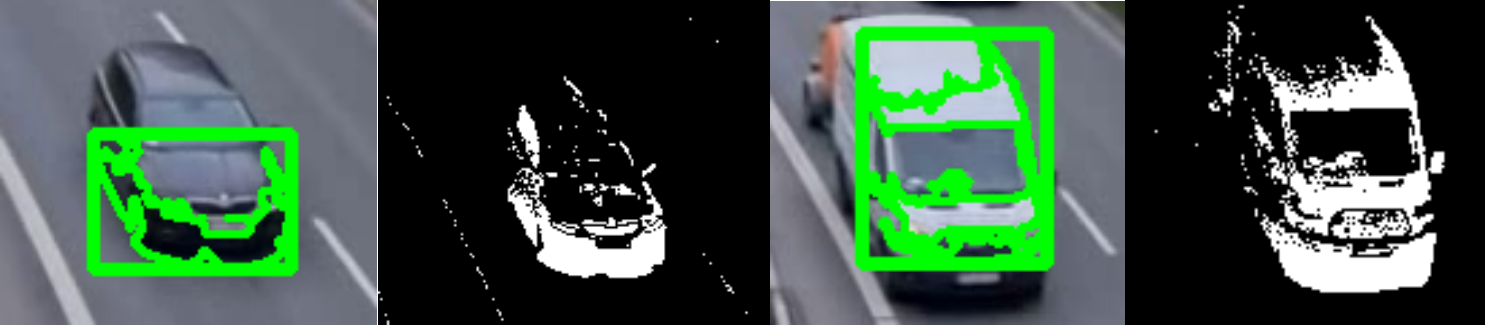
\includegraphics[width=8cm]{Media/MOGVergleich.png}
			\caption{Schwierigkeiten bei der Objekterkennung}
			\label{mogFehler}
		\end{center}
	\end{figure}
	+++++++++++++++++Streifenproblem...++++++++
	
	\section{Objekterkennung: YoloV4}
	YOLO ist ein Neuronal Netz für die Echtzeit-Objekterkennung. In diesem Projekt wurde die vierte und damit aktuellste Version von Yolo\cite{b2} verwendet. So bietet jede Version inkrementelle Verbesserung zum jeweiligen Vorgänger. In dem folgenden Abschnitt werden die wichtigsten Punkte aller Versionen erläutert.\\
	YOLO ist die Abkürzung für 'You Only Look Once' was übersetzt 'Man sieht nur einmal hin' heißt. Die Aufgabe der Objekterkennung besteht darin, den Ort und die Größe der Bounding Box im Bild zu bestimmen, sowie die Objekte zu klassifizieren. Frühere Methoden, wie R-CNN und seine Variationen, verwendeten eine Pipeline, um diese Aufgabe in mehreren Schritten durchzuführen. Dies ist in der Ausführung langsam und aufwendiger zu trainieren, da jede einzelne Komponente separat trainiert werden muss. YOLO, erledigt beide Aufgaben mit einem einzigen Convolutional Neural Network. Es betrachtet dabei die Objekterkennung als ein Regressionsproblem auf räumlich getrennte Bounding Boxes und zugehörige Klassenwahrscheinlichkeiten.\\
	Für die Regression verwendete Loss-Funktion betrachtet drei Komponenten:
	\begin{enumerate}
		\item \textbf{Localization loss:} Differenz zwischen vorhergesagten Bounding-Box-Werten (x,y,w und h) und tatsächlichen Bounding-Box-Werten.
		\[ \lambda_{coord} \sum_{i=0}^{S^2}\sum_{j=0}^{B} \mathbb{1}_{i j}^{obj} [(x_i - \hat{x}_i )^2 + (y_i - \hat{y}_i )^2] \]
		\[ + \lambda_{coord} \sum_{i=0}^{S^2}\sum_{j=0}^{B} \mathbb{1}_{i j}^{obj} [(\sqrt{w_i} - \sqrt{\hat{w}_i} )^2 + (\sqrt{h_i} - \sqrt{\hat{h}_i} )^2] \]
		Wenn $\mathbb{1}_{i}^{obj} = 1$ dann ist die Boundingbox $j$ in Zelle $i$ verantwortlich das Objekt zu erkennen. $\lambda_{coord}$ ist eine Gewichtung um den Localization loss wichtiger zu machen. Standardmäßig ist $\lambda_{coord} = 5$ \cite{b5}.
		
		\item \textbf{Confidence loss:} Fehler im Konfidenzwert.
		\[  \sum_{i=0}^{S^2}\sum_{j=0}^{B} \mathbb{1}_{i j}^{obj} (C_i - \hat{C}_i)^2 \]
		$\hat{C}_i$ ist der Konfidenzwert der Boundingbox $j$ in Zelle $i$. Wenn $\mathbb{1}_{i}^{obj} = 1$ dann ist die Boundingbox $j$ in Zelle $i$ verantwortlich das Objekt zu erkennen.\\
		Wenn das Objekt nicht erkannt wurde ist der Confidence loss:
		\[  \lambda_{noobj} \sum_{i=0}^{S^2}\sum_{j=0}^{B} \mathbb{1}_{i j}^{noobj} (C_i - \hat{C}_i)^2 \]
		$\lambda_{noobj}$ ist eine Gewichtung um den Confidence loss unwichtiger zu machen. Standardmäßig ist $\lambda_{noobj} = 0.5$ \cite{b5}.
		
		\item \textbf{Classification loss:} Differenz zwischen den vorhergesagten Klassenwahrscheinlichkeiten und den tatsächlichen Klassenwahrscheinlichkeiten:
		\[ \sum_{i=0}^{S^2} \mathbb{1}_{i}^{obj} \sum_{c \in classes} (p_i(c) - \hat{p}_i(c))^2 \]
		Wenn $\mathbb{1}_{i}^{obj} = 1$ dann wurde ein Objekt in Zelle $i$ gefunden.
		$\hat{p}_i(c)$ beschreibt die Klassenwahrscheinlichkeit für die Klasse $c$ in der Zelle $i$ \cite{b5}.
	\end{enumerate}
	Zusammengesetzt sieht der Loss wie folgt aus:
	\[ \lambda_{coord} \sum_{i=0}^{S^2}\sum_{j=0}^{B} \mathbb{1}_{i j}^{obj} [(x_i - \hat{x}_i )^2 + (y_i - \hat{y}_i )^2] \]
	\[ + \lambda_{coord} \sum_{i=0}^{S^2}\sum_{j=0}^{B} \mathbb{1}_{i j}^{obj} [(\sqrt{w_i} - \sqrt{\hat{w}_i} )^2 + (\sqrt{h_i} - \sqrt{\hat{h}_i} )^2] \]
	\[ + \sum_{i=0}^{S^2}\sum_{j=0}^{B} \mathbb{1}_{i j}^{obj} (C_i - \hat{C}_i)^2 \]
	\[ + \lambda_{noobj} \sum_{i=0}^{S^2}\sum_{j=0}^{B} \mathbb{1}_{i j}^{noobj} (C_i - \hat{C}_i)^2 \]
	\[ + \sum_{i=0}^{S^2} \mathbb{1}_{i}^{obj} \sum_{c \in classes} (p_i(c) - \hat{p}_i(c))^2 \]
	Das Bild ist in ein S × S-Gitter mit den Residualblöcken aufgeteilt. Wenn der Mittelpunkt eines Objekts in eine Gitterzelle fällt, ist diese Gitterzelle für die Erkennung dieses Objekts zuständig. Jede Gitterzelle sagt B Bounding Boxes und C Klassenkonfidenzwerte für diese Boxen voraus \cite{b1}\\
	Diese Klassenkonfidenzwerte zeigen, wie sicher das Modell ist, dass die Boundingbox ein Objekt enthält und auch wie genau die Box das Objekt beschreibt. Die Konfidenz wird wie folgt definiert:
	\[ c = Pr(Objekt) * IoU_{pred}^{truth} \]
	Die IoU ist zwischen zwei Boxen A und B ist wie folgt definiert:
	\[ IoU = \frac{A \cap B}{A \cup B} \]
	\begin{figure}[h]
		\begin{center}
			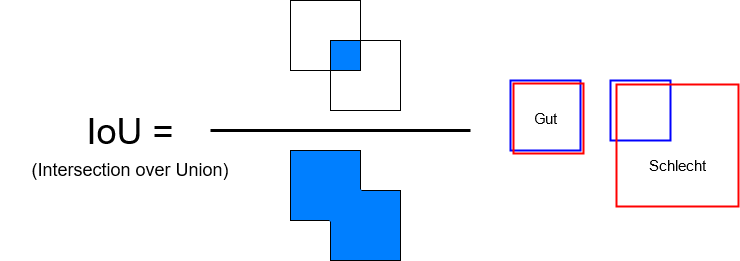
\includegraphics[width=8cm]{Media/Iou.png}
			\caption{Intersection-Over-Union}
			\label{IoU}
		\end{center}
	\end{figure}\\
	In Abbildung \ref{IoU} ist die Berechnung der Intersection-Over-Union dargestellt. Sie beschreibt das Verhältnis der Schnittfläche einer Bounding Box mit der Grundwahrheit bezüglich der Gesamtfläche von Bounding Box und Grundwahrheit. Je genauer die beiden Flächen übereinander liegen desto höher der Wert, desto besser ist die Vorhersage der Bounding Box.\\
	\\
	In der zweiten Version von Yolo wurde an mehreren Stellen Verbesserungen erreicht. So wurde beispielsweise Batch-Normalization in Convolutional-Layers eingefügt.\\
	Die Inputgröße des Netzes wurde von $224*224$ auf $448*448$ erhöht.\\
	Eine weitere wichtige Änderung sind Ankerboxen. Da Objekte meist immer ähnliche Formen haben kann eine gewisse Menge an sogenannten Ankerboxen definiert werden, welche als Basis Boundingboxen fingieren. So wird anstatt die absolute Größen von Boxen in Bezug auf das gesamte Bild vorherzusagen, eine Ankerbox ausgewählt die am besten zu dem gewünschten Objekten passende verwendet. Die Abbildung \ref{Anker} zeigt dieses Konzept.
	\begin{figure}[!h]
		\begin{center}
			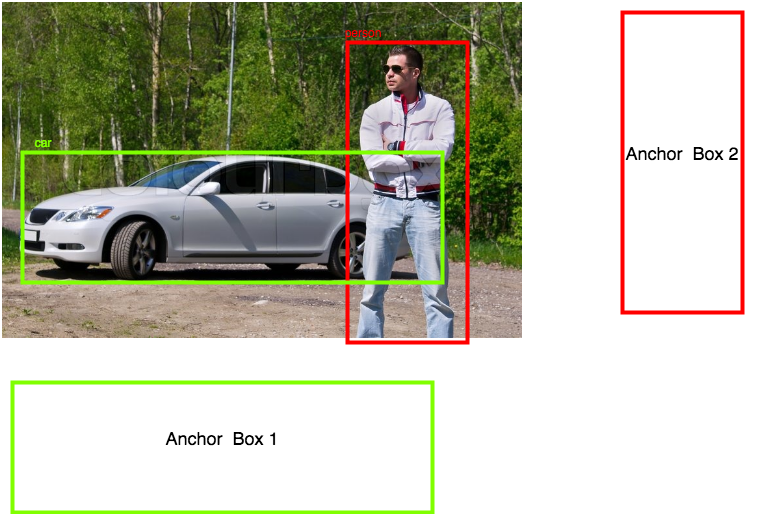
\includegraphics[width=6cm]{Media/Ankerboxen.png}
			\caption{Passende Ankerboxen werden ausgewählt\cite{b0}}
			\label{Anker}
		\end{center}
	\end{figure}
	Diese Ankerboxen kann man mittels Clusteralgorithmen wie K-Means und den Boundingboxen aus dem Datensatz berechnen. Dies hat vor allem den Vorteil, dass die Boundingboxen besser zu den Objekten des jeweiligen Datensatzes passen.\\
	Jede Vorhersagen für eine Boundingbox enthält die 4 Koordinaten: $t_x, t_y, t_w, t_h$. $t_x$ und $ t_y$ sind die x an y Koordinaten, relative Zellen Mittelpunkt. $t_w$ und $ t_h$ sind die Skalierungsfaktoren relativ zu Ankerboxdimensionen. $p_w$ und $p_h$ sind die Breite und Höhe der Ankerbox. Dabei gibt es noch einen Gitterzellenoffset $c_x$ und $c_y$.
	\begin{figure}[!h]
		\begin{center}
			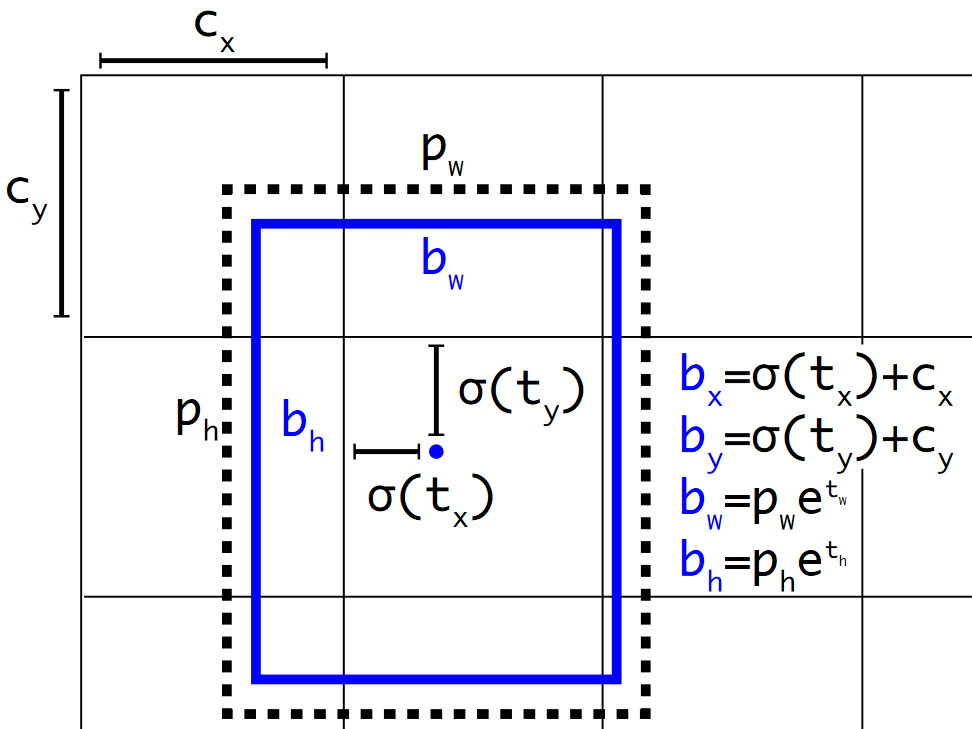
\includegraphics[width=6cm]{Media/YoloV3PredictionBox.png}
			\caption{Zusammensetzung einer Boundingbox\cite{b3}}
			\label{PredictionBox}
		\end{center}
	\end{figure}\\
	Außerdem wir der \textit{objectness score} $t_o$ vorhergesagt.
	\[ P_r(Object)*IoU_{b}^{object} = \sigma(t_o) \]
	$\sigma(t_o)$ entspricht dem Box Konfidenz Score.
	Der Output des Modells enthält für jede Gitterzelle n Boxen, wobei n der Anzahl der Ankerboxen entspricht. Jede Box ist ein Vektor aus vier Koordinaten, dem \textit{Objectnessscore} und der Klassenwahrscheinlichkeiten C. Der Vektor enthält: $[b_x,b_y,b_w,b_h, b_o, C]$\cite{b3}.
	\[ C = [c_1, c_2,..., c_{80}]^T\]
	\[ P = [P_r * c_1, P_r * c_2, ..., P_r * c_{80}] \]
	\[ class = argmax_i(C)\]
	\[ score = max(P)\]\\
	In der dritten Version wurde vor allem die Genauigkeit weiter verbessert. So wurden Restblöcke, Skip-Verbindungen und Upsampling Techniken hinzugefügt. Das Netzwerk wuchs damit drastisch auf insgesamt 106 Convolutional-Layer.
	Der Featureextraktor Darknet19 aus YoloV2 wurde durch Darknet-53 ersetzt. Darknet-53 besitzt 53 Convolutional-Layer und beinhaltet zusätzlich vereinzelte Abkürzungen im Netz.\\
	Eine weitere Änderung betrifft den Softmax-Layer für die Bestimmung der Zielklasse. Früher wurde nur die Klasse ausgewählt, die den höchsten Score erzielte. Dies hat sich geändert. Dadurch, dass die Klassenvorhersage mit Hilfe einer Logistische Regression stattfindet, kann ein Objekt mehrere Label gleichzeitig haben wie zum Beispiel Person und Frau. Diese Multilabelklassifikation wird für unser Projekt aber nicht benötigt.\\
	Ein weitere Neuerung ist das Vorhersagen über drei verschiedener Skalierungen. Das System extrahiert Merkmale mit einem ähnlichen Konzept wie bei Merkmalspyramidennetzen (FPN). Diese Technik verbessert die Genauigkeit vor allem bei kleineren Objekten. So werden Feature-Map aus einer früheren Schicht aus dem Netzwerk extrahiert und mit höher gesampelten Features durch Verkettung zusammen gefügt. Mit weiteren Faltungsschichten werden diese kombinierte Feature-Map verarbeitet. So wird von Vorhersagen für alle der drei Skalierungen profitiert und damit von allen vorherigen Berechnungen, sowie von den feinkörnigen Merkmalen aus der frühen Phase des Netzwerks. Die Abbildung \ref{FPN} zeigt das Konzept eines Merkmalspyramidennetzwerks.
	\begin{figure}[!h]
		\begin{center}
			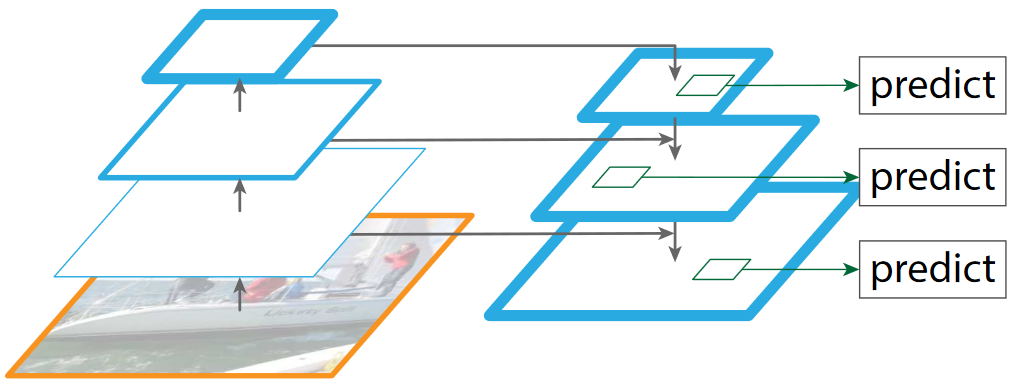
\includegraphics[width=6cm]{Media/FPN.png}
			\caption{Darstellung eines Merkmalspyramidennetzwerks \cite{b6}}
			\label{FPN}
		\end{center}
	\end{figure}\\
	Die letzte dieser Schichten der jeweiligen Skalierungen sagt einen 3-D-Tensor voraus, der Bounding Box, Objekthaftigkeit und Klassenvorhersagen enthält. Es werden aber für jede der drei Skalierung drei Boxen vorausgesagt. Der Tensor enthält dann die vier Bounding-Box-Offsets, eine Objektvorhersage und 80 Klassenvorhersagen $N*N*[3*(4 + 1 + 80)]$ \cite{b4}.\\
	\\
	YoloV4 hat die Geschwindigkeit und Genauigkeit verbessert. So nennt das Paper \cite{b2} zum Beispiel \textit{Bag of Freebies}. Damit sind Verbesserungen gemeint die die Genauigkeit des Modells zur Trainingszeit verbessern, aber die Inferenzzeit nicht beeinflussen. So wurde stark das Training optimiert. Bei dem Training werden Bilder zusätzlich aus dem Datensatz generiert. Existierende Bilder werden dupliziert und dann rotiert, zugeschnitten, verzerrt, verdunkelt, etc. und dann auch durch das Netz geschickt. 
	Auch Techniken wie \textit{Cut Mix} und \textit{Mosaic Dataaugmentation} werden angewendet. Bei älteren Verfahren werden Bildteile gelöscht. Bei den beiden verwendeten Verfahren werden stattdessen Bildteile aus den Trainingsdaten ausgeschnitten und kombiniert, wobei die Ground-Truth-Labels ebenfalls angepasst werden müssen. Die Data Augmentation sorgt für eine verbesserte Generalisierungfähigkeit des Modells.\\
	Regularisierungsmethoden wie \textit{DropOut} und \textit{DropBlock} wurden gegen Overfitting eingesetzt.\\
	Auch wird die Lossfunktion aus YoloV1 angepasst. Bei den bisherigen Versionen wurde die mittlere quadratische Abweichung (MSE) für das Regressionsproblem verwendet. Die Regression wird dann unabhängig für alle Vorhersagen von $t_x, t_y, t_w, t_h$ verwendet. Sinnvoller ist es die Koordinaten zusammen als die IoU der Boundingboxen in Betracht zu ziehen. Deshalb verwendet YoloV4 \textit{CIoU} als Lossfunktion, um die Integrität der Objekte mit einzubeziehen.\\
	Weitere Verbesserungen die auf Kosten der Laufzeit gehen werden \textit{Bag of Specials} genannt. Dazu gehören zum Beispiel \textit{Squeeze-and-Excitation}, \textit{Spatial Attention Module}, Vergrößerung des Rezeptionsfeldes des Modells und Stärkung der Fähigkeit zur Merkmalsintegration.\\
	Im Backbone wird eine \textit{MISH}-Aktivierungsfunktion verwendet. Diese ist eine glatte und nicht-monotone neuronale Aktivierungsfunktion, die wie folgt definiert werden kann:
	\[ f(x) = x* \tanh (\ln (1+e^x)) \]
	Sie arbeitet besser als zum Beispiel \textit{ReLU} oder Swish \cite{b7}.\\
	Die Komponenten in der Architektur wurde auch ersetzt. Im \textit{Backbone} läuft nun \textit{CSPDarknet53}. Dies basiert auf dem Darknet53 aus YoloV3 und wird mit Cross-Stage-Partial-Networks erweitert. Im Hals des Netzes wird \textit{Spatial pyramid pooling} (SPP) verwendet. \textit{Path Aggregation Network} (PANet) und \textit{Spatial Attention Module} (SAM) ersetzen die Merkmalspyramidennetze (FPN) die YoloV3 verwendet.\\
	\textit{Convolutional-Layer} brauchen keine feste Bildgröße und erzeugen deshalb  Feature-Maps beliebiger Größe. \textit{Fullyconnected-Layer} benötigen stattdessen per Definition eine Eingabe mit fester Länge. SPP entfernt genau diese Restriktion. SPP wendet verschiedene Strategien bei unterschiedlichen Skalierungen an. Die Feature-Maps werden räumlich in $m$ × $m$ Bins unterteilt. Dann wird ein Maximumpool auf jeden Bin für jeden Kanal angewendet. In YoloV4 wird eine modifiziert Version von SPP verwendet die die räumliche Dimension der Ausgabe beibehaltet \cite{b9}.\\
	In den FPN aus YoloV3 werden die Objekte separat und unabhängig voneinander auf verschiedenen Skalenebenen erkannt. Dies kann zu doppelten Vorhersagen führen. PAN erweitert FPN mit einem Bottom-up-Pfad der die Weitergabe von Informationen aus den unteren Ebenen erleichtern. Durch adaptives Featurepooling kann auf jede Vorhersagen aus allen Ebenen zugriffen werden.\cite{b10}\\
	SAM verbessert die räumliche Aufmerksamkeit.\\
	Am \textit{Head} der für Prädiktion verantwortlich ist wurde nichts geändert und  ist damit identisch zu YoloV3 \cite{b2}\cite{b8}. Diese Architektur mit der Vielzahl an Komponenten wird in er Abbildung \ref{V4Arch} dargestellt.
	\begin{figure}[!h]
		\begin{center}
			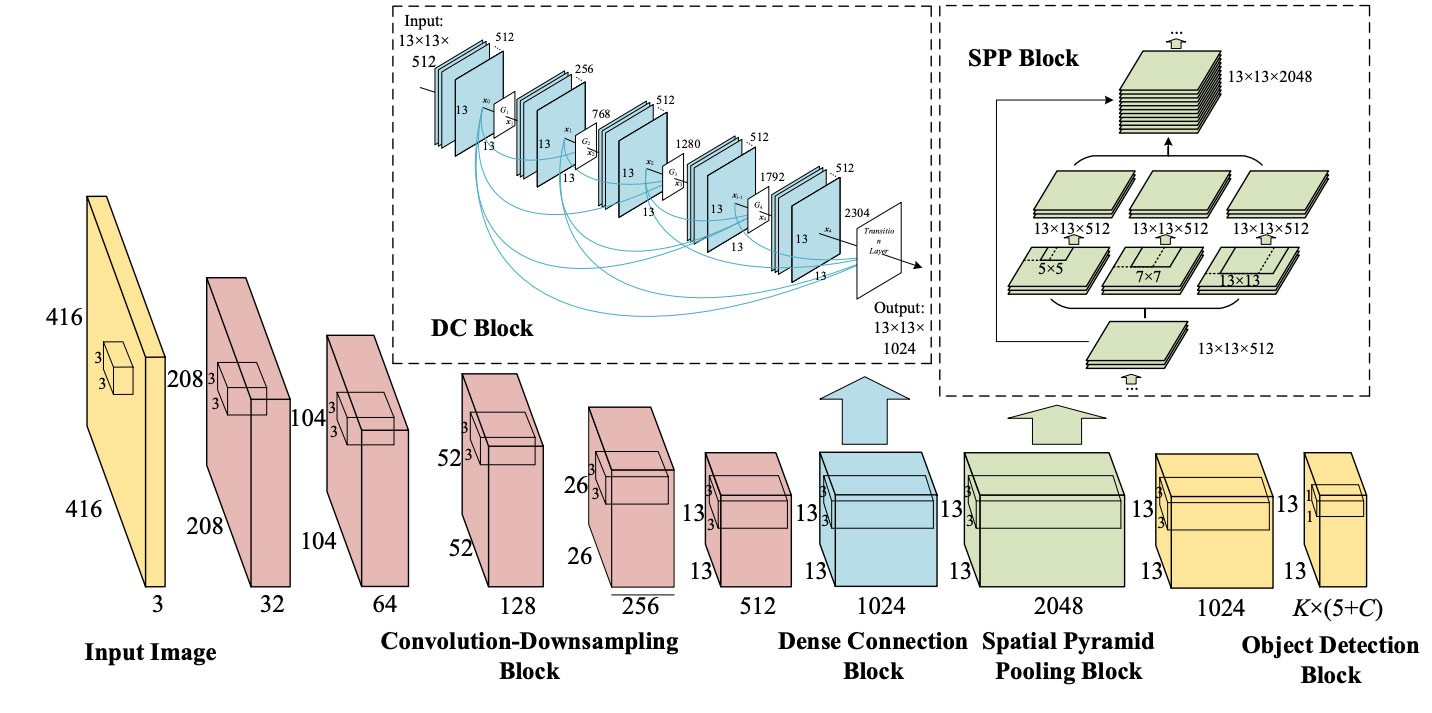
\includegraphics[width=9cm]{Media/YoloV4Arch.jpeg}
			\caption{Das Konzept von YoloV4 \cite{b8}}
			\label{V4Arch}
		\end{center}
	\end{figure}\\
	Wir mussten unser Modell nicht mehr trainieren da es bereits mit dem Microsoft COCO Datensatz trainiert wurde. Es sind 80 verschiedene Klassen erkennbar. Wir interessieren uns aber nur für einen kleineren Teil wie:
	\begin{enumerate}
		\item Personen
		\item Pkw
		\item Lkw
		\item Busse
		\item Fahrräder
		\item Züge
	\end{enumerate}
	Das Modell könnte noch besser arbeiten, wenn es nur auf die Klassen trainiert würde die für unser Projekt relevant sind. Dies hätte aber den Rahmen des Projektes gesprengt. Das Modell ist mit ein paar Ausnahmen für das Projekt ausreichend gut genug.\\
	Dennoch kann man je nach Szenario per Parameter die relevanten Klassen auswählen. Das Modell prädiktiert trotzdem noch alle Klassen. Die nicht relevanten werden im Postprocessing herausgefiltert.\\
	Ein weitere Postprocessingschritt ist es die Detektion die eine zu geringe Sicherheit besitzen zu entfernen.\\
	Die übrigen Boxen durchlaufen eine Non-Maximum-Suppression.
	Der Output kann überschneidende Boundingboxen besitzen die eigentlich zur selben Klasse gehören. Diese Duplikate können mittels der Non-Maximum-Suppression (NMS) entfernt werden. Hierfür wird die IoU der Boxen berechnet. Sollte die IoU einen Threshold überschreiten dann wird das Duplikat entfernt. Die Grafik \ref{NMS} zeigt wie zu viele überlappende Boxen mit einer NMS mit einer ersetzt werden kann.\\
	\begin{figure}[!h]
		\begin{center}
			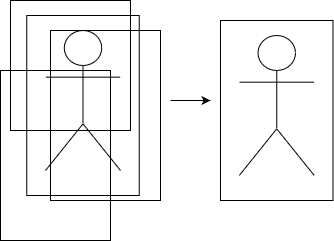
\includegraphics[width=6cm]{Media/NMS.png}
			\caption{Non-Maxima-Suppression}
			\label{NMS}
		\end{center}
	\end{figure}\\
	Das Ergebnis einer Prädiktion ist eine Liste von Objekten, welche aus den x,y Koordinate des Mittelpunktes der Boundingbox, der Breite w, der Höhe h, der Klasse und des Konfidenzwerts besteht.
	
	\subsection{Fehler in der Erkennung}
	YoloV4 ist nicht perfekt. So gibt es gelegentlich Falschklassifizierungen, fehlende Detektionen oder unpassende Boundingboxen.  Fehlerursachen sind aber sehr schwer zu erklären, da das Netz eine Blackbox ist. Dieser Abschnitt zeigt Beispiele für diese Art von Fehler auf.\\
	\textbf{Falschklassifizierung:}\\
	Selten Klassifiziert das Netz falsch. So wie in der Abbildung \ref{FaK} zu sehen ist wurde ein Bus als Pkw klassifiziert. Das Modell ist sich in diesem Beispiel auch nur unsicher mit $31\%$. Der Fehler lässt sich vermutlich erklären da die Frontpartie des Bus einem Pkw sehr ähnelt und der Rest des Fahrzeuges wegen eines Baum und einer Laterne verdeckt wird. Auch ist zu vermuten, dass das Netz falsche Merkmale gelernt hat. Dies könnte mit Sicherheit verbessert werden wenn das Modell nur auf die für das Projekt relevanten Klassen trainiert worden wäre. Die folgenden Abbildungen \ref{FaK}, \ref{FaK2}, \ref{FaK3} und \ref{FaK4} sind Beispiele für falsche Klassifikationen. Speziell ist vor allem der Fehler in Bild \ref{FaK4}. Hier wurde ein Anhänger als Fahrzeug klassifiziert. Der Ursprung dieses Fehlers kann unterschiedliche Gründe haben. Dies liegt wahrscheinlich auch am Datensatz selbst.
	\begin{figure}[!h]
		\begin{center}
			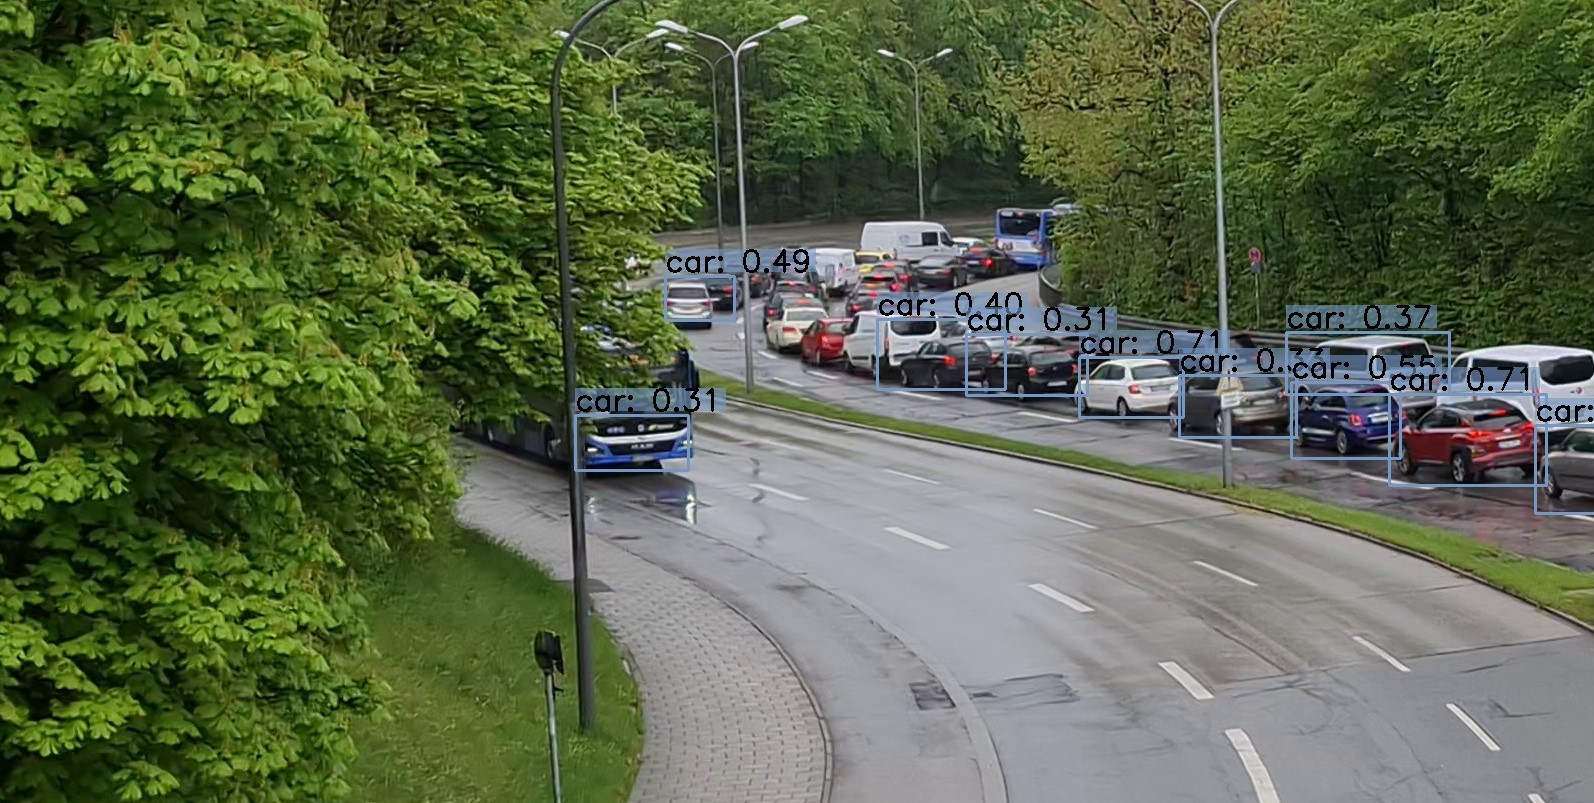
\includegraphics[width=7cm]{Media/Output_480 - Kopie.jpg}
			\caption{Falschklassifizierung eines Bus wegen Verdeckung}
			\label{FaK}
		\end{center}
	\end{figure}
	\begin{figure}[!h]
		\begin{center}
			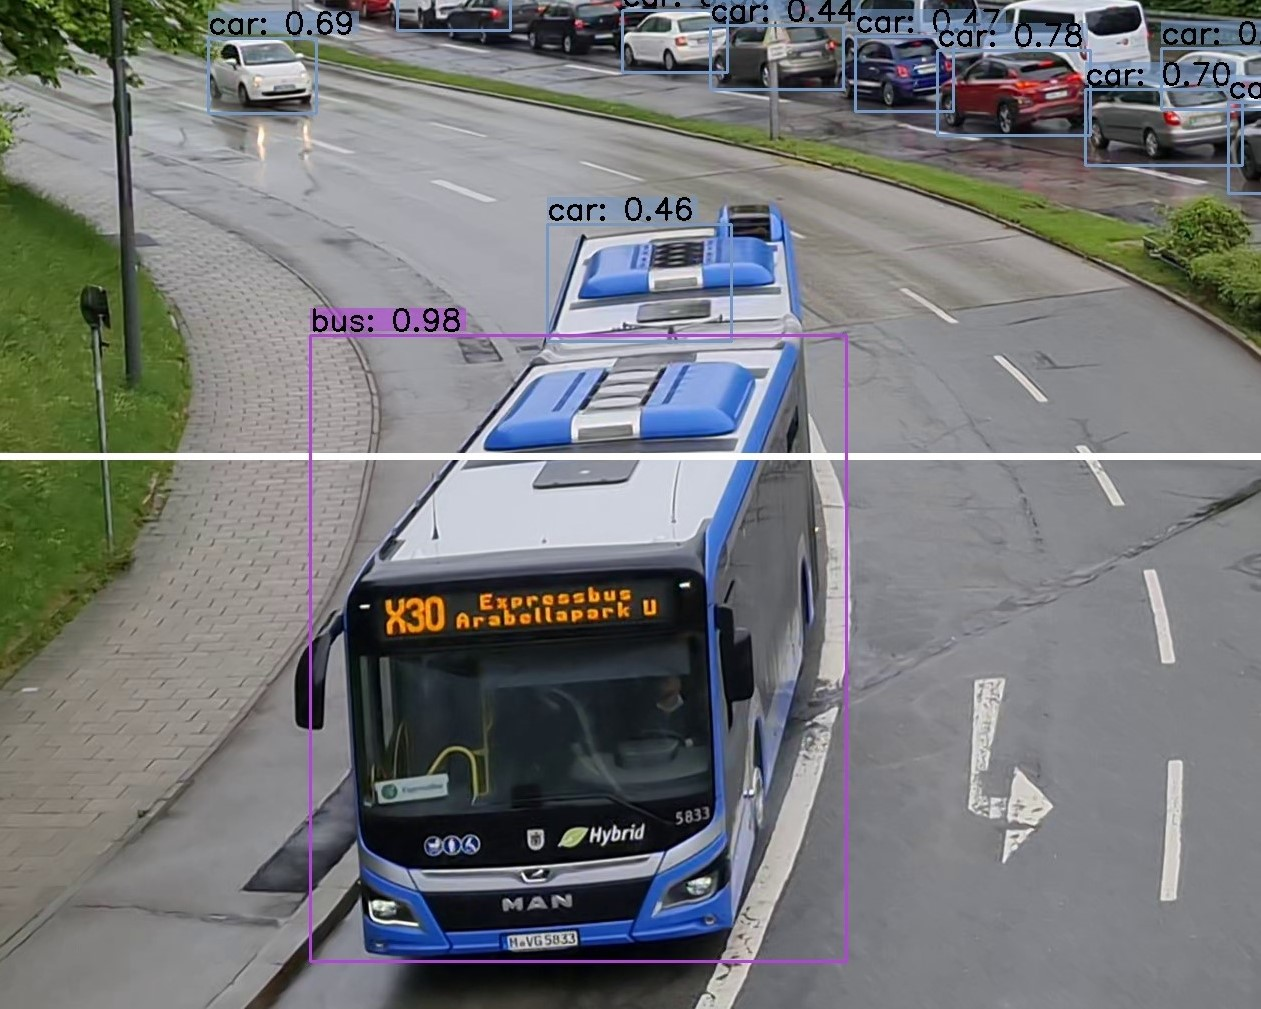
\includegraphics[width=7cm]{Media/Output_847 - Kopie.jpg}
			\caption{Falschklassifizierung des Dachs als Pkw}
			\label{FaK2}
		\end{center}
	\end{figure}
	\begin{figure}[!h]
		\begin{center}
			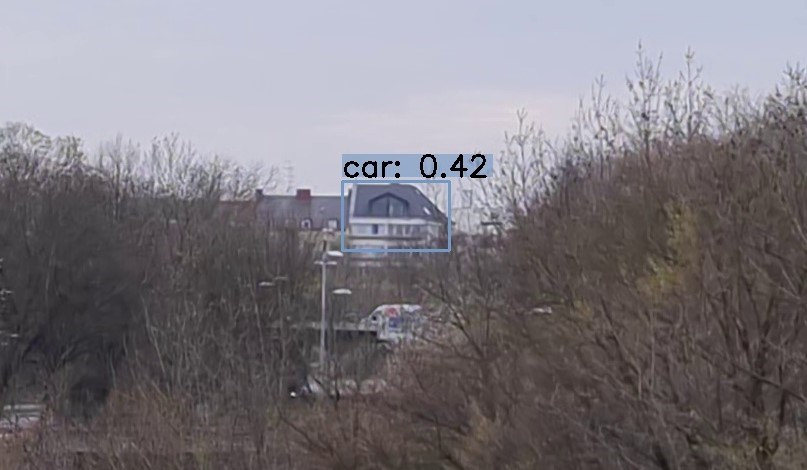
\includegraphics[width=7cm]{Media/Output_108 - Kopie (2).jpg}
			\caption{Falschklassifizierung eines Hausdachs}
			\label{FaK3}
		\end{center}
	\end{figure}
	\begin{figure}[!h]
		\begin{center}
			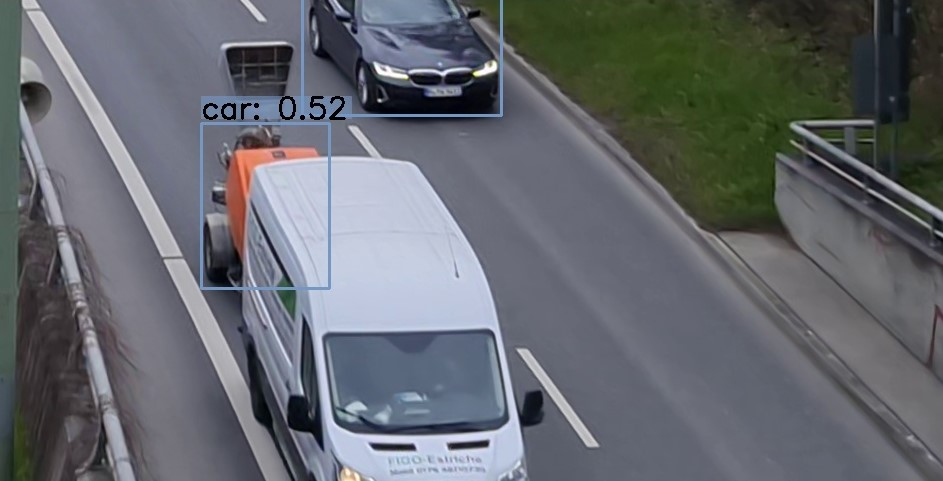
\includegraphics[width=7cm]{Media/Output_829 - Kopie.jpg}
			\caption{Falschklassifizierung eines Anhängers}
			\label{FaK4}
		\end{center}
	\end{figure}\\
	
	\textbf{Fehlende Detektion:}\\
	Ein etwas häufigerer Fehler ist das Detektionen komplett fehlen. So zeigt die Abbildung \ref{FeK} und \ref{FeK2} zwei Typische Gründe. Hauptgrund ist es das Objekte teilweise verdeckt sind. In Kombination, wenn Objekte sehr klein sind, ist es nahezu nicht mehr möglich zuverlässig Detektion zu bekommen. Auch wenn Objekte das Bild verlassen oder gerade betreten kann es noch kurz zu fehlenden Detektionen führen.
	\begin{figure}[!h]
		\begin{center}
			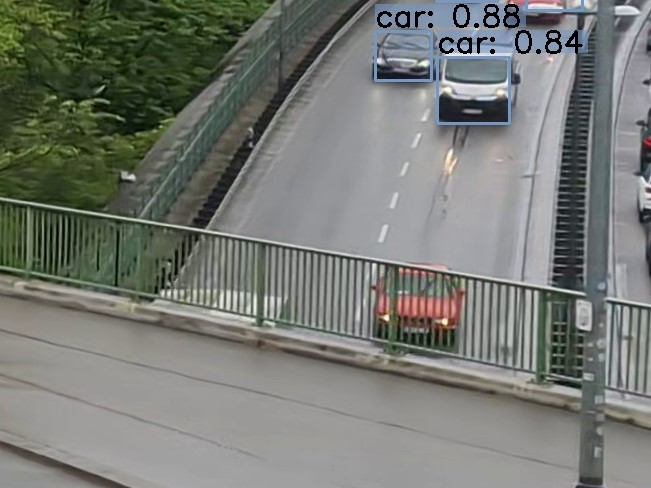
\includegraphics[width=7cm]{Media/Output_680 - Kopie.jpg}
			\caption{Fehlende Klassifikationen}
			\label{FeK}
		\end{center}
	\end{figure}\\
	\begin{figure}[!h]
		\begin{center}
			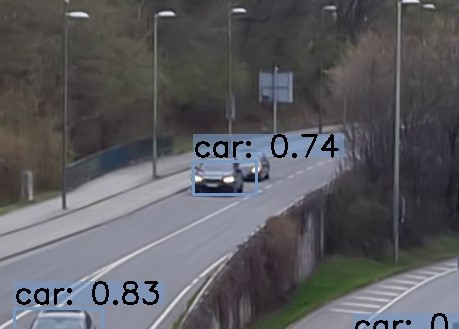
\includegraphics[width=7cm]{Media/Output_108 - Kopie.jpg}
			\caption{Fehlende Klassifikationen}
			\label{FeK2}
		\end{center}
	\end{figure}\\
	\textbf{Unpassende Boundingboxen:}\\
	Yolo hat durch seine Eigenschaft nur rechteckige Boundingboxen vorhersagen zu können eine große Schwäche. Das resultiert in manchen Szenarien zu sehr unpassenden Boundingboxen. Beispielsweise kann man in der Abbildung \ref{UB} gut erkennen das wegen dem Busses welcher Diagonal steht die Boxen sehr groß werden können. Der Effekt tritt noch verstärkter auf bei noch längere Objekten wie Zügen wie zum Beispiel in Bild \ref{UB4} zusehen. Der Fehler der in Abbildung \ref{UB3} zu sehen ist hängt womöglich von Fehlern im Training zusammen. Züge wurden vielleicht an Bahnsteigen schlecht gelabelt was dem Netz dann beigebracht hat Bahnsteige als Züge zu klassifizieren. Auch kann die Box für das Objekt etwas falsch anliegen wenn Bäume oder Laternen ein Teil verdecken wie in Abbildung \ref{UB2} zu sehen ist. Diese unpassenden Boxen erschweren das Tracking ungemein. Dazu später aber noch mehr. 
	\begin{figure}[!h]
		\begin{center}
			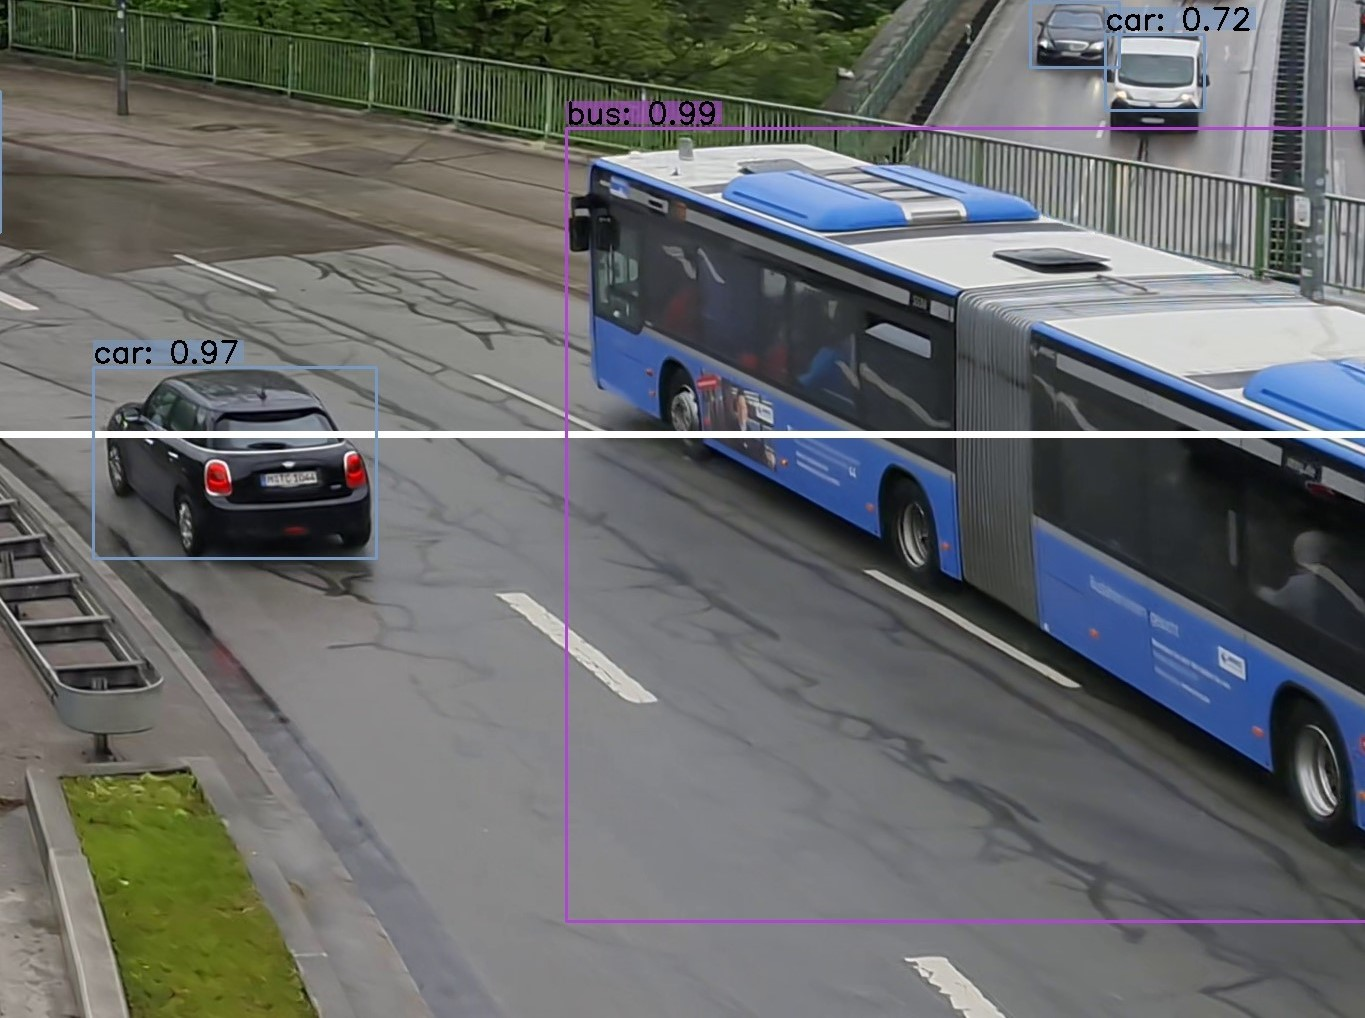
\includegraphics[width=8cm]{Media/Output_777 - Kopie.jpg}
			\caption{Unpassende Boundingbox}
			\label{UB}
		\end{center}
	\end{figure}\\
	\begin{figure}[!h]
		\begin{center}
			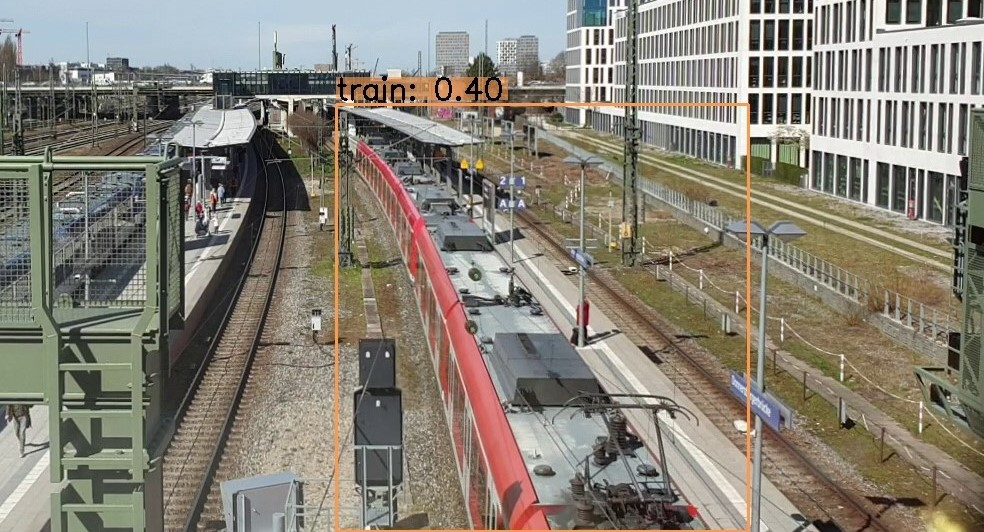
\includegraphics[width=8cm]{Media/Output_2126.jpg}
			\caption{Unpassende Boundingbox}
			\label{UB4}
		\end{center}
	\end{figure}\\
	\begin{figure}[!h]
		\begin{center}
			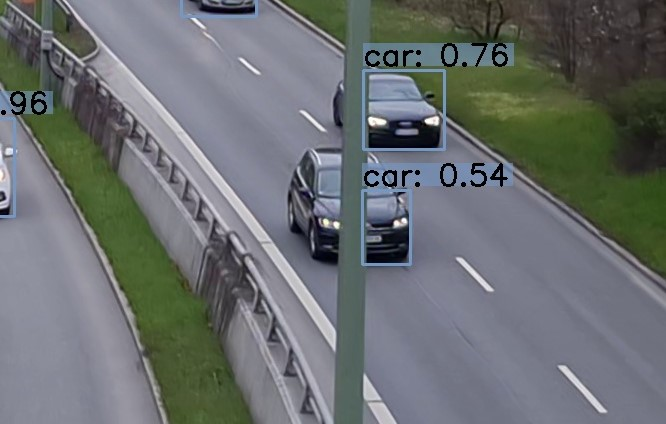
\includegraphics[width=8cm]{Media/Output_276 - Kopie.jpg}
			\caption{Unpassende Boundingbox}
			\label{UB2}
		\end{center}
	\end{figure}\\
	\begin{figure}[!h]
		\begin{center}
			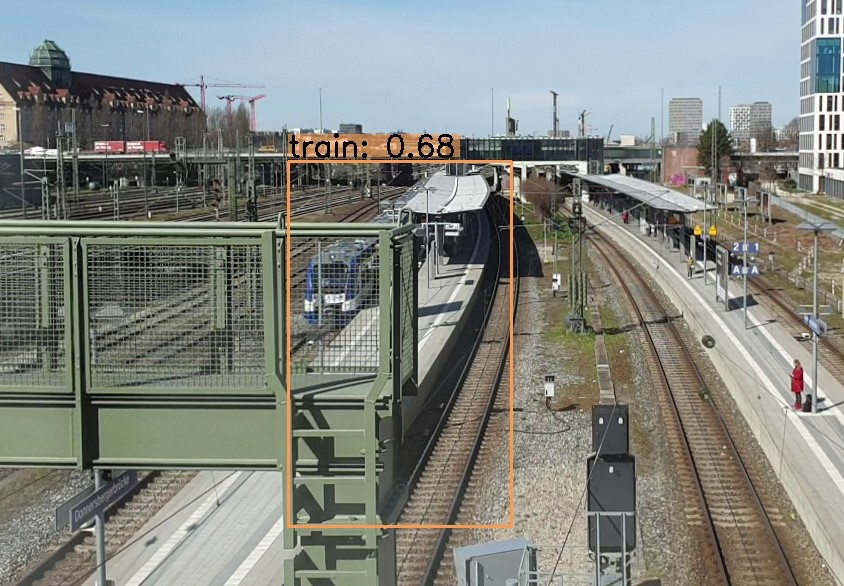
\includegraphics[width=8cm]{Media/Output_564.jpg}
			\caption{Unpassende Boundingbox}
			\label{UB3}
		\end{center}
	\end{figure}\\

	
	
	\section{Tracking: Sort}
	SORT berechnet auf Basis des Kalman Filters und der Hungarian Methode die Bewegung des Objekts und weist je nach Status eine eindeutige Identifikationsnummer zu. 
	
	Der Kalman-Filter funktioniert für die Problemstellung sehr gut, da dieser ein lineares System mit gaußisches Rauschen voraussetzt. Dies ist gegeben durch die gleichmäßige Bewegung der Züge/ Autos in eine Richtung.
	Der Kalmanfilter kann aus verrauschten, teils redundanten Messungen die Zustände und Parameter des aktuellen Systems schätzen. 
	Die Zustände des aktuellen Systems sind die Positionen der Objekte angegeben in Bounding Boxen. Durch Berücksichtigung des letzten Zustand des Systems, (die letzte Position), der Schätzung der nächsten Position und Abgleich mit der aktuellen Messung (die aktuelle Detektion) und anschließender Aktualisierung des Systems, kann eine zuverlässige Verfolgung des Objekts berechnet werden. Probleme die den Kalmanfilter stören sind zum Beispiel ungleichmäßige Bewegungen von Fahrzeugen, dies wird „Process Noise“ genannt, sowie Ungenauigkeiten in Messungen, diese werden als „Measurement Noise“ bezeichnet.
	Kann zu dem aktuell getrackten Objekt in dem Frame keine Bounding Box zugeordnet werden, wird der Zustand des Systems auch ohne die Korrektur durch die Messung berechnet. Kann in einem späteren Frame wieder eine Bounding Box zugeordnet werden, wird der Zustand durch diese Detektion erneut aktualisiert.
	
	Die Hungarian Methode wird verwendet, um die Detektion einem existierenden getrackten Objekt zuzuordnen. Hierfür wird die Intersection-over-Union Distance zwischen jeder Detektion und allen bereits erkannten Objekten verglichen und als Gewichtung verwendet.
	
	Die Zuweisung der ID erfolgt anschließend über die optimale Lösung der Hungarian Methode, auch Kuhn-Munkres-Algorithmus genannt. Diese wird für das Lösen von Zuordnungsproblemen in einem gewichteten kompletten bipartiten Graph genutzt. Hierbei wird die Zuordnung anhand der minimalen Gewichtung, zwischen den Elementen gelöst. Gegeben ist ein Graph $G = (A \cup B, E) $. Zwischen $A$ und $B$ wird nun die Verbindung mit der kleinsten Gewichtung gesucht. Hierfür wird eine Kostenmatrix $C$ erstellt mit $c_{ij}$ als Kosten um $a_i \in A$, $b_j \in B$ zuzuordnen. Die Matrix $C$ wird anschließend reduziert. In diesem Beispiel werden Objekte den Detektionen zugeordnet. Als Gewichtung dienen die Distanzen der IoU, welche minimal sein soll.
	 
	 ++++++++Fehler SORT++++++++++++
	 
	\section{Tracking: DeepSort}
	
	SORT an sich ist bereits ein Tracker, das Problem ist jedoch, dass die ID-Änderungen zu oft auftreten. Das heißt die Objekt-ID wechselt während der Verfolgung. Ausgelöst wird dies zum Beispiel durch die teilweise Verdeckung des Objekts. Deshalb wurde SORT um ein CNN erweitert, welches sowohl einerseits die Mahalanobis-Distanzmetrik für die Assoziation nutzt, als auch die Form des Objekts in Form eines durch das hinzugefügte CNN berechneten Feature-Vektor verfolgt. Durch Verwendung einer geeigneteren Distanzmetrik und Beschreibung des Objekts kann dieses nun besser verfolgt werden.
	Das CNN erstellt einen Vektor, der enthält alle Features eines gegebenen Bilds. Ursprünglich wird das Neuronale Netz als Klassifikator trainiert. Indem die Klassifikations Layer weggelassen werden, können die resultierenden Feature-Vektoren als Wiedererkennungsform verwendet werden.
	
	Anstatt bei der Ungarischen Methode wie bei SORT die IoU-Distanz zu verwenden, wird diese durch die (quadrierte) Mahalanobis Distanz ersetzt. Die Mahalanobis Distanz berechnet den Abstand von einem Punkt zu einer Verteilung. Der Abstand ist dabei wie viele Standardabweichungen der Verteilung dieser Punkt vom Mittelwert der Verteilung entfernt ist. Er wird somit durch die Standardabweichung der Verteilung normiert. Die Detektion stellt hierbei den Punkt da und die Unsicherheit der Zustandsvorhersage, beziehungsweise die Unsicherheit der Position des getrackten Objekts, die Verteilung. Dadurch wird bei der Berechnung der Distanz die Unsicherheit der Position miteinbezogen. 
	Die Mahalanobis Distanz berechnet in dieser Anwendung die Distanz zwischen der detektierten Bounding Box und der gaußverteilten Vorsage des Zustands des Kalman-Filters:
	\begin{align}
		d^{(1)}(i,j)= (d_j - y_i)^TS^{-1}_i(d_j - y_i)
	\end{align}
	Hierbei wird die Verteilung, zuvor acht-dimensional des i-ten verfolgen Objekts in den vier-dimensionalen Raum der Messungen projiziert $(y_i, S_i)$. Diese Bounding Box der Detektion wird mit $d_j$ bezeichnet. \\
	
	
	\begin{tabular}{r l}
		Kalman-Filter Zustand: & $(u,v,\gamma,h,\dot{x},\dot{y},\dot{\gamma},\dot{h})$ \\
		Detektion: & $(u,v,\gamma,h)$ \\
		$u,v$ :& Mittelpunkt der Bounding Box \\
		$h$ :& Skalierungsfaktor \\
		$\dot{x},\dot{y},\dot{\gamma},\dot{h}$: & Geschwindigkeiten in Bild- \\	
		& koordinaten \\
	\end{tabular} \\
	
	Ist die Bewegung des Objekts nicht linear steigt die Unsicherheit in der Vorhersage der Position durch den Kalman-Filter. Treten zudem Bewegungen durch die Kamera auf, kommt es zu starken Verschiebungen innerhalb der Bildebene. Die Mahalanobis Distanz ist lediglich für Bewegungen mit geringer Unsicherheit geeignet, wodurch die Nutzung dieser Metrik für die Verfolgung verdeckter Objekte ungeeignet ist, da hier die Bewegungsunsicherheit besonders groß ist.
	Es wird daher eine weitere Metrik eingeführt, welche die Form der Objekte vergleicht. Die Beschreibung ist ein Feature-Vektor, welcher durch ein CNN berechnet wird. 
	
	Für die Distanzmetrik ergibt sich dann folgende Gleichung
	$D = \lambda * D_k + (1-\lambda) * D_a$. Hierbei ist $D_k$ die Mahalanobis Distanz und $D_a$ die kleinste Kosinus-Distanz zwischen den Feature-Vektoren. $\lambda$ dient als ein Gewichtungsfaktor.
	
	Kann DeepSORT erfolgreich ein bereits verfolgtes Objekt zu einer Detektion assoziieren, wird anschließend eine TrackingID erstellt. Hierbei muss beachtet werden, dass im Zuge der Verbesserung von SORT weitere Sicherheiten eingebaut wurden. Ein neu getracktes Objekt erhält nicht sofort eine endgültige Identifikationsnummer. Erst nachdem das Objekt in drei hintereinander liegenden Frames erfolgreich getrackt werden konnte erhält es eine Nummer. Das Objekt erhält des weiteren einen Zähler $a$, der die Anzahl an Frames zählt, seitdem das Objekt nicht mehr erfolgreich assoziiert werden konnte. Ist eine maximale Anzahl $Age_{max}$ erreicht gilt das Objekt als verloren oder außer Reichweite der Kamera und wird aus der Objektliste entfernt. Dieser Zähler wird jedoch zurückgesetzt, sollte zuvor das Objekt erneut erfolgreich assoziiert werden.
	
	\subsubsection{Ergebnisse des Tracking mit DeepSORT}
	Das Tracking basiert auf YOLO, daher wird es beeinträchtigt wenn YOLO Objekte nicht erkennt. Der Kalman-Filter kann zwar in Fällen von fehlenden Detektionen weiterhin eine Vorhersage liefern, allerdings nur bei gleichbleibender Bewegung in eine Richtung. 
	
	Geprüft wurde wie lange der Tracker erfolgreich stehende und fahrende Autos verfolgen kann. In den meisten Fällen ist dabei kein Problem festzustellen. Problematisch ist, wenn der Objekt-Detektor über mehrere Frames ein Objekt nicht erkennt.
	
	In den Aufzeichnung des Brudermühl-Tunnels zeigt sich die Problematik der
	unregelmäßigen Detektionen deutlich. Ein Teil der Straße wird durch die Laterne
	verdeckt, wodurch für einige Frames keine Detektion möglich ist. Die Fahrzeuge
	erhalten eine neue ID. Nachdem die Laterne jedoch passiert wurde wird die alte
	Nummerierung teilweise wieder zurückgesetzt, sodass lediglich eine Unterbrechung
	erfolgt.
	
	Des weiteren entfernt sich teilweise das Fahrzeug zu schnell während die Bounding Boxen fehlen und kann nicht
	mehr der zuvor festgelegten Tracking-ID zugeordnet werden. Hierbei wird ebenfalls eine neue ID zugewiesen.
	
	Objekte können durch zu schnelle Bewegung die ID des zuvor sich an der Stelle
	befindenden Objekts übernehmen, dies ist zu sehen in Abbildung \ref{track4}-\ref{track6}.
	Dabei wechselt Fahrzeug 6 auf die ID 69. Da ist im Abbildung \ref{track5} wieder zurück auf 6
	wechselt ist die ID 69 offen. Da Fahrzeug 63 für kurze Zeit hinter der Laterne keine Bounding Box erhält, wird fälschlicherweise die ID 69 zugewiesen.
	Dies wird in der nächsten Abbildung \ref{track6} nicht mehr korrigiert, da es sich zu schnell entfernt.
	
	\begin{figure}[!h]
		\begin{center}
			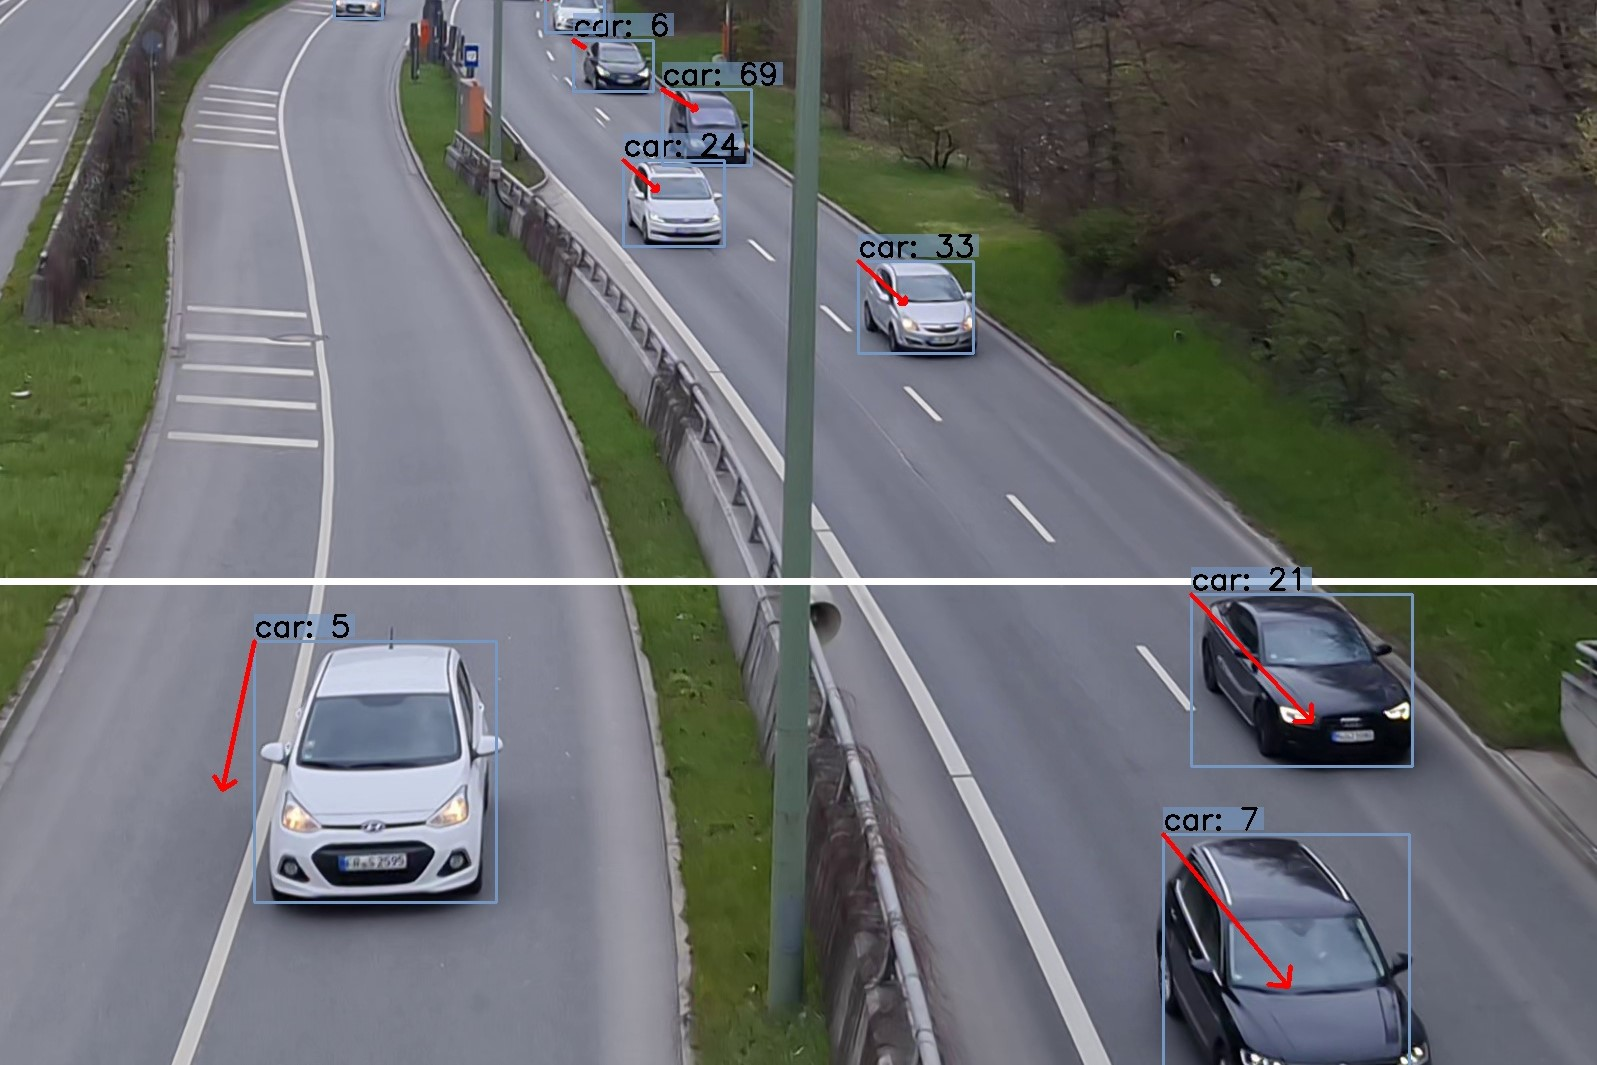
\includegraphics[width=7cm]{Media/switch1.jpg}
			\caption{Im Hintergrund zu sehen Auto 6, 24 und 48 die die Lampe passieren}
			\label{track3}
		\end{center}
	\end{figure}
	\begin{figure}[!h]
		\begin{center}
			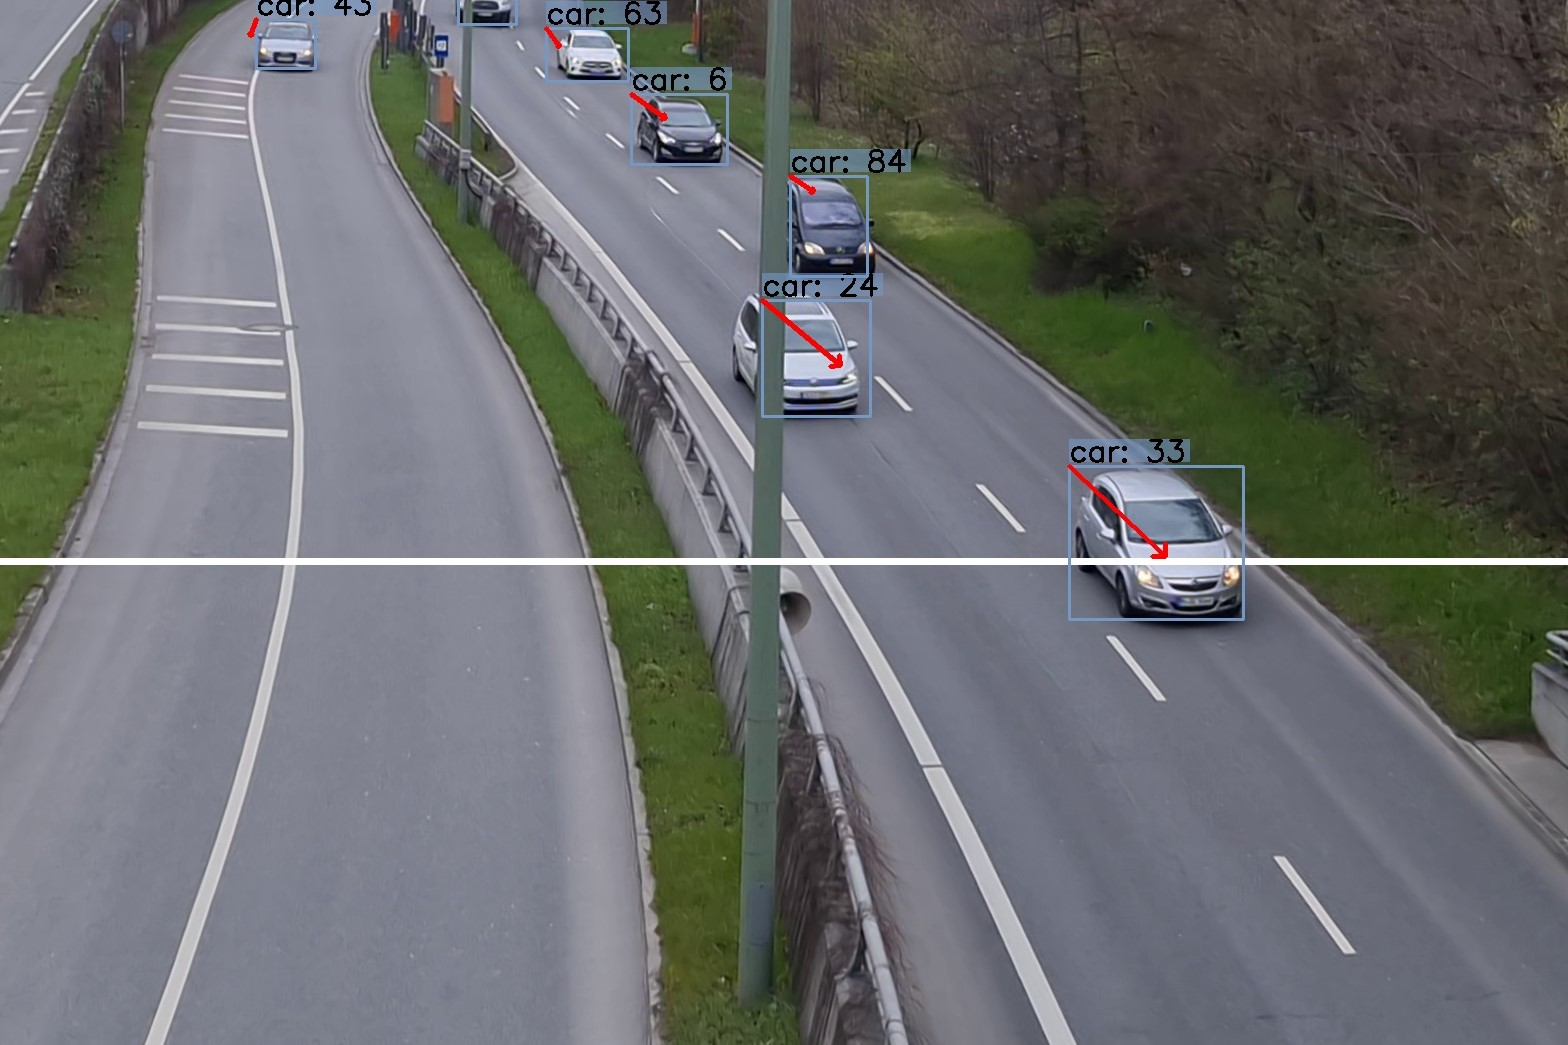
\includegraphics[width=7cm]{Media/switch2.jpg}
			\caption{Tracken nach passieren der Lampe von 24 und 48 erfolgreich, wechselt der ID von Auto 6 auf 69, Fahrzeug 63 im Hintergrund}
			\label{track4}
		\end{center}
	\end{figure}
	\begin{figure}[!h]
		\begin{center}
			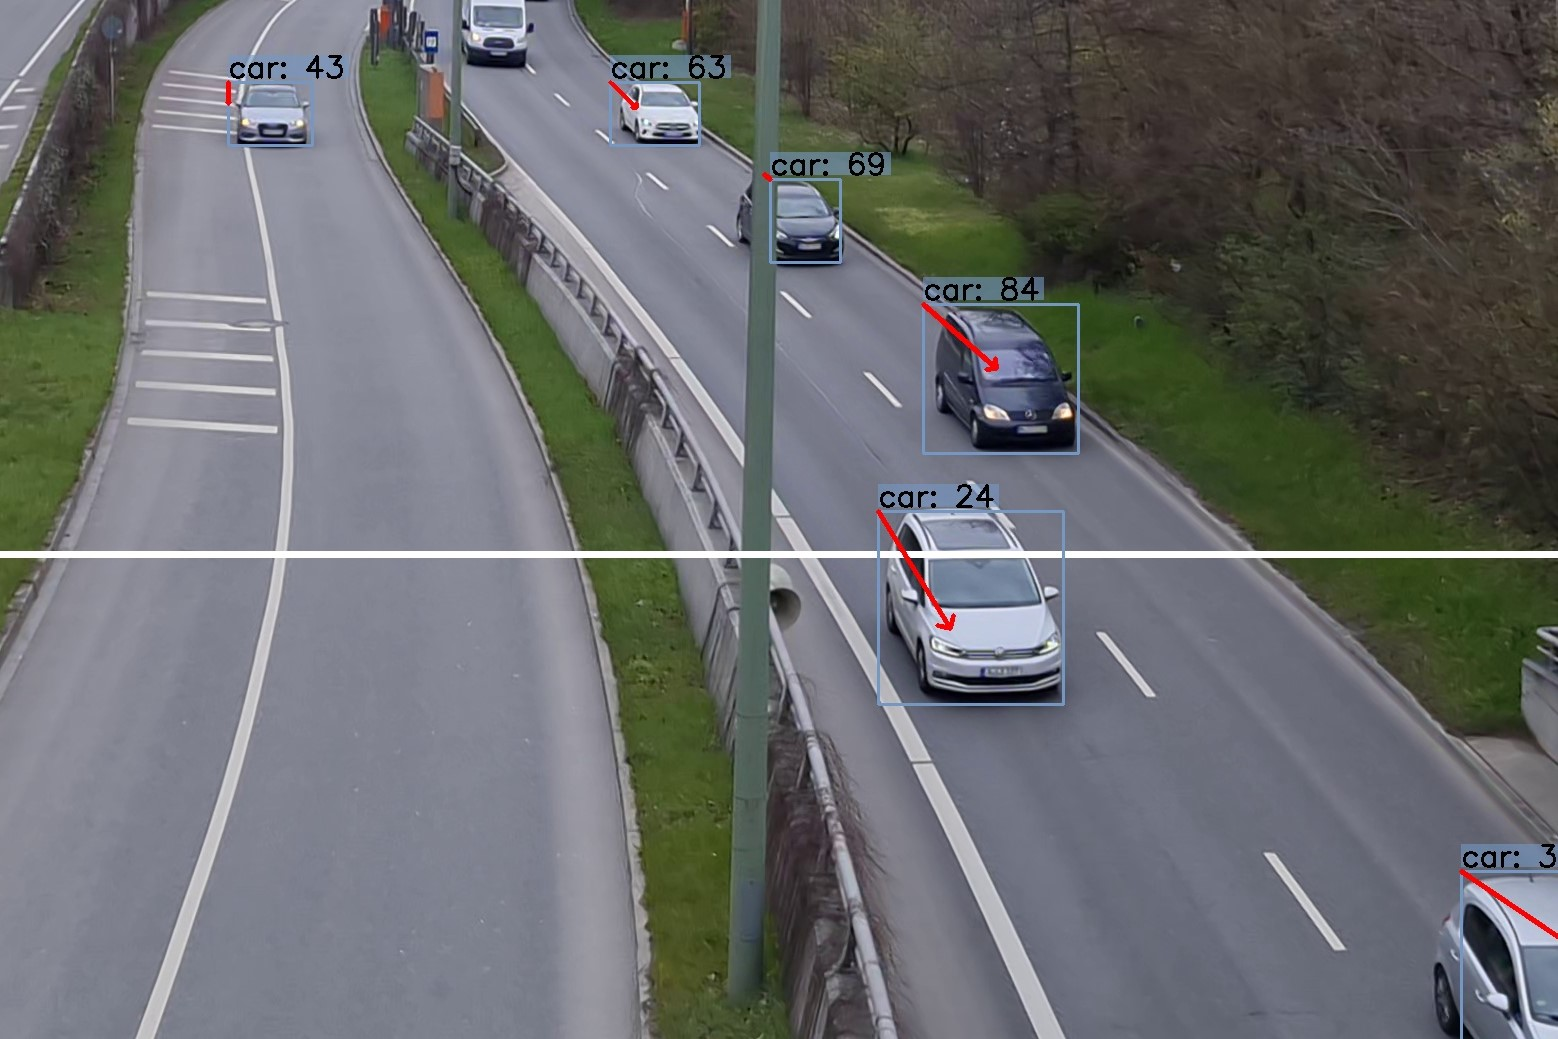
\includegraphics[width=7cm]{Media/switch3.jpg}
			\caption{Wechselt von ursprünglich 6 von 69 zurück auf 6 }
			\label{track5}
		\end{center}
	\end{figure}
	\begin{figure}[!h]
		\begin{center}
			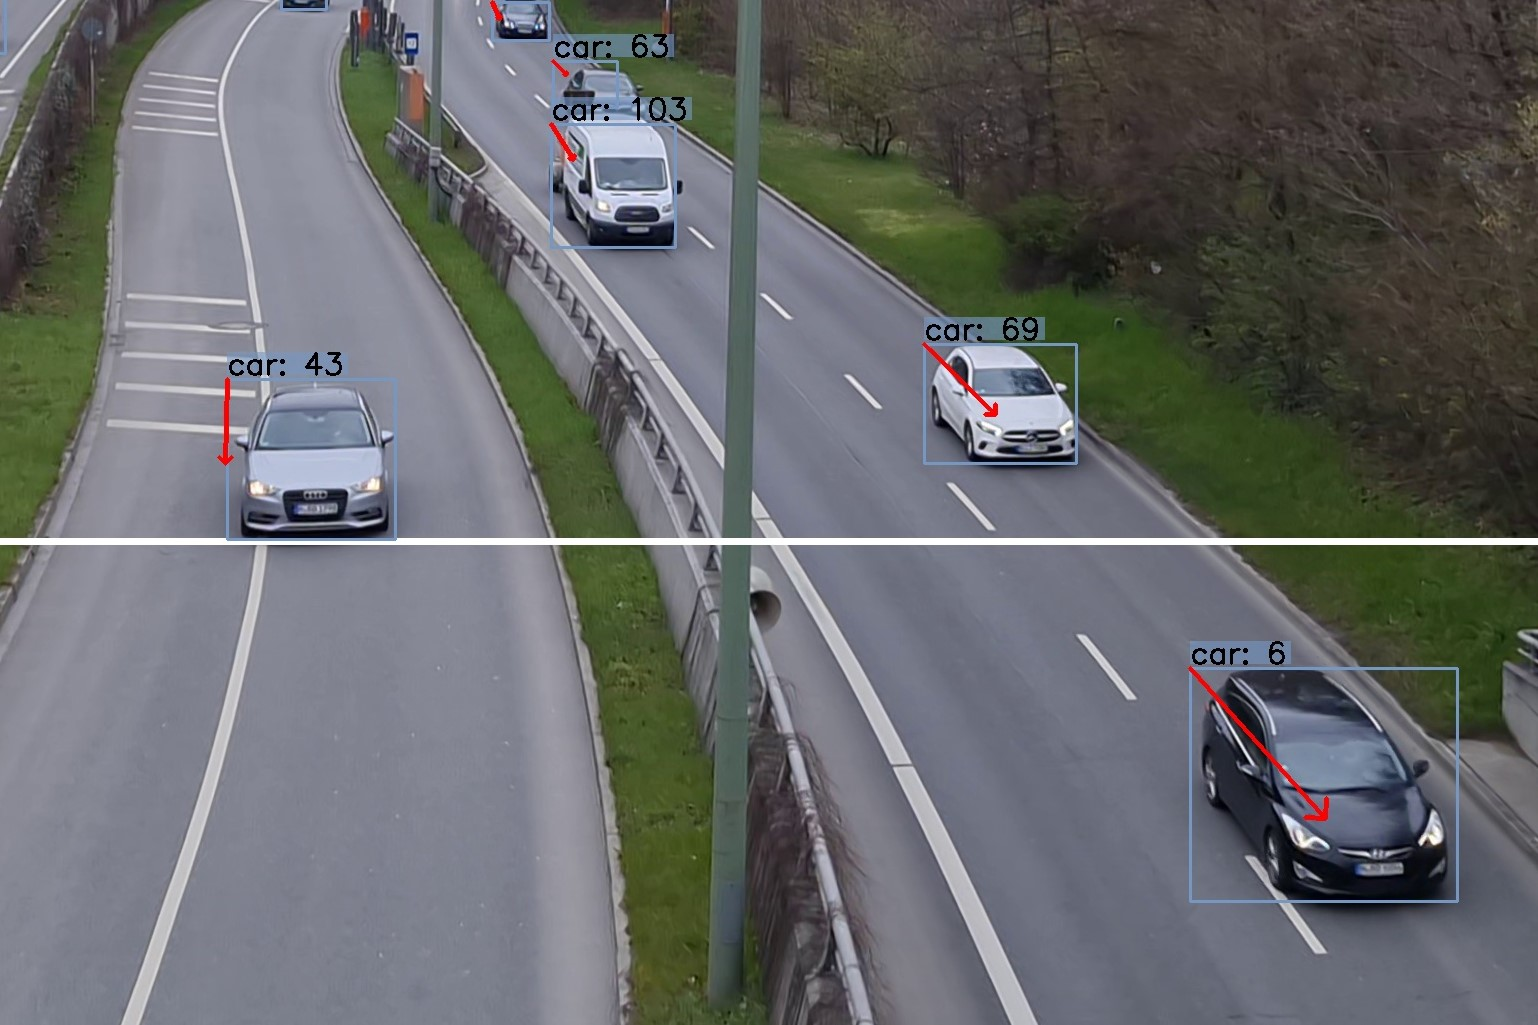
\includegraphics[width=7cm]{Media/switch4.jpg}
			\caption{Wechsel von Fahrzeug 63 auf 69, dahinterliegende Fahrzeug erhält 63}
			\label{track6}
		\end{center}
	\end{figure}
	
	
	In den Aufzeichnungen des Candid-Tunnels zeigen sich Probleme bei der Verfolgung von weiter entfernten und stehenden Fahrzeugen.
	
	Die Verfolgung der nahen stehenden Fahrzeuge funktioniert gut, allerdings kommt es zu
	häufigen Änderungen der ID bei den weiter entfernten stehenden Fahrzeugen.
	Nahe sich bewegende Fahrzeuge können zuverlässig verfolgt werden, ebenfalls die sich gleichmäßig weiter entfernten. Im Bild groß erscheinende und sich bewegende Objekte können zuverlässig verfolgt werden.
	
	Stehende Fahrzeuge mit fehlenden Detektionen erhalten neue IDs nach mehreren
	Frames. Die vorherigen IDs werden zu schnell verworfen, wodurch neue IDs erstellt werden.
	Der Wechsel auf neue IDs ist in den Abbildungen \ref{track1} bis \ref{track2} 
	gezeigt.
	
	\begin{figure}[!h]
		\begin{center}
			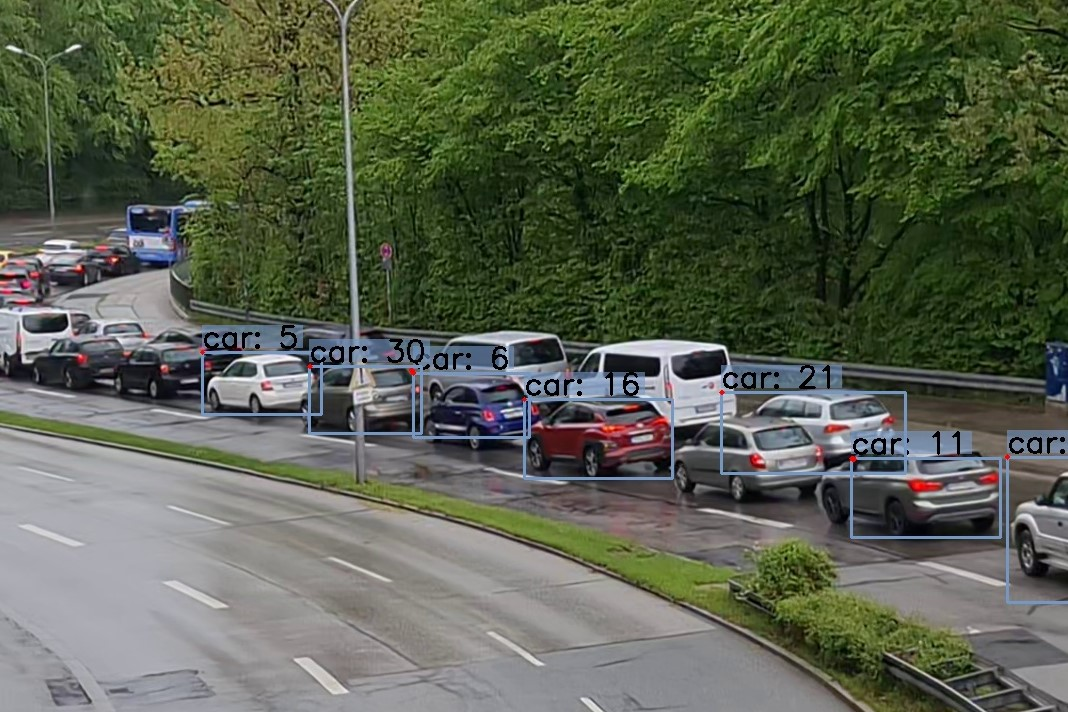
\includegraphics[width=7cm]{Media/track1.jpg}
			\caption{Track-ID bei stehenden Fahrzeuge 6 und 30}
			\label{track1}
		\end{center}
	\end{figure}
	\begin{figure}[!h]
		\begin{center}
			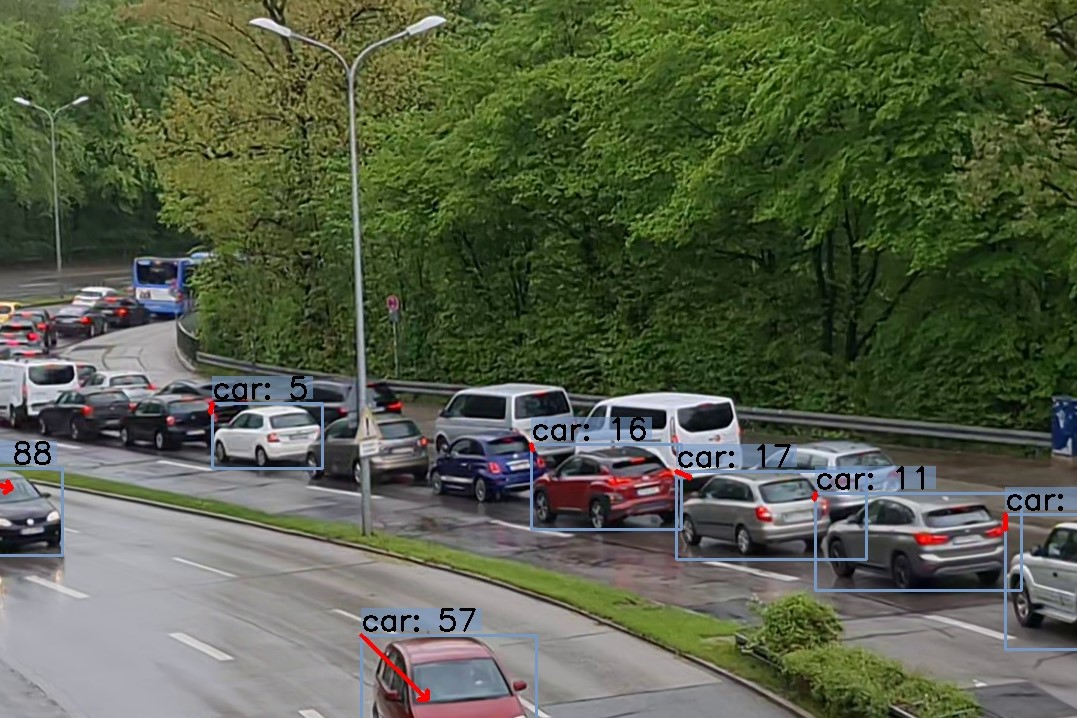
\includegraphics[width=7cm]{Media/track3.jpg}
			\caption{Keine Detektion der Fahrzeuge 6 und 30}
			%Hier ebenfalls zu sehen fehlende Erkennungen
			\label{track1.5}
		\end{center}
	\end{figure}
	\begin{figure}[!h]
		\begin{center}
			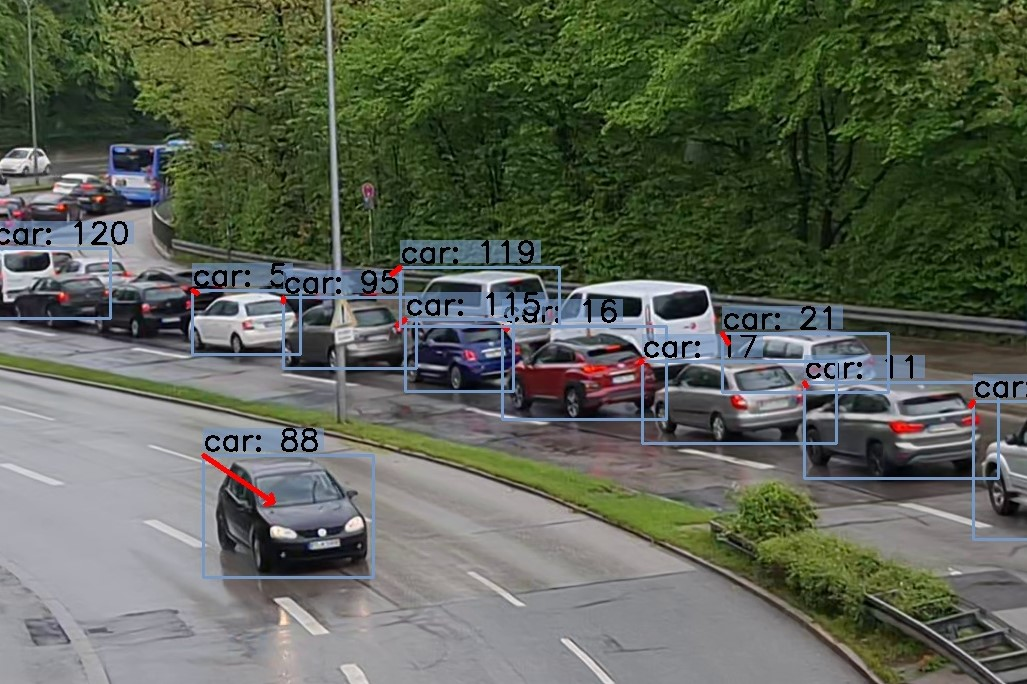
\includegraphics[width=7cm]{Media/track2.jpg}
			\caption{Änderung der Track-ID bei stehenden Fahrzeugen - 6 und 30 wechseln zu 95 und 115}
			%Hier ebenfalls zu sehen fehlende Erkennungen
			\label{track2}
		\end{center}
	\end{figure}
	
	In den Abbildungen \ref{LLost1}-\ref{LLost3} ist der Verlust der ID des blauen Trucks zu
	beobachten. Gleichzeit zeigt der Richtungspfeil in die entgegengesetzte Richtung. Hier
	versagt der Kalman-Filter in der Richtungsbestimmung. Die Vorhersage kann nicht
	mehr der Detektion zugeordnet werden und eine neue ID wird gewählt
	
	\begin{figure}[!h]
		\begin{center}
			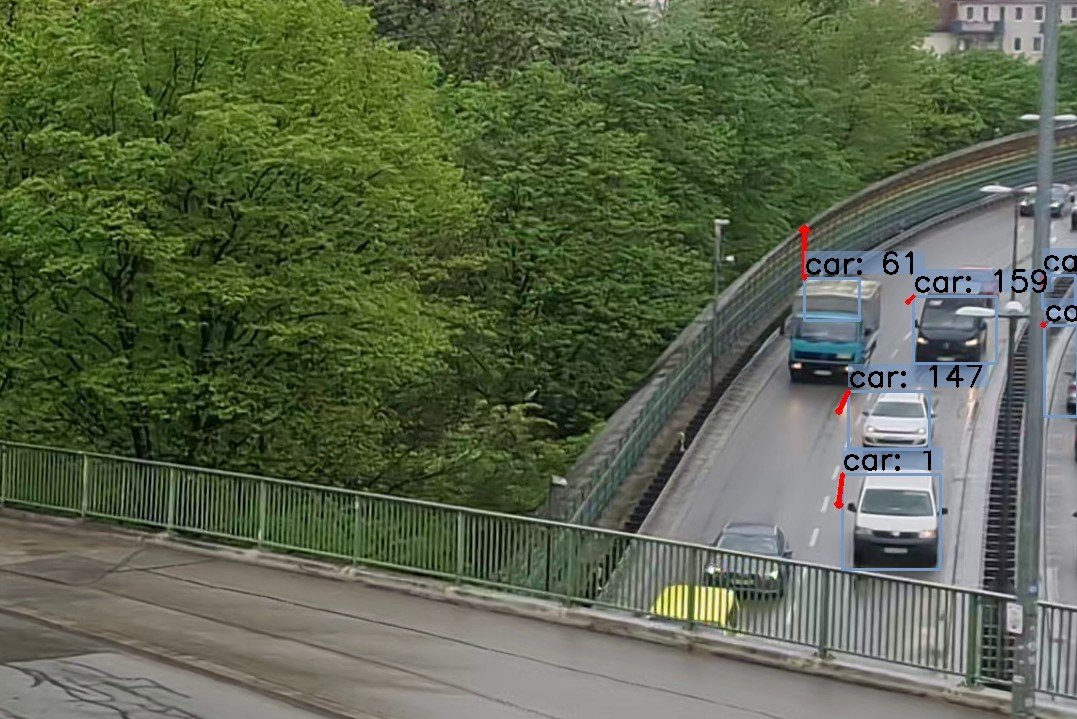
\includegraphics[width=7cm]{Media/LLost1.jpg}
			\caption{Fahrzeug mit ID 61, Richtungspfeil zeigt in entgegengesetzte Richtung}
			\label{LLost1}
		\end{center}
	\end{figure}
	\begin{figure}[!h]
		\begin{center}
			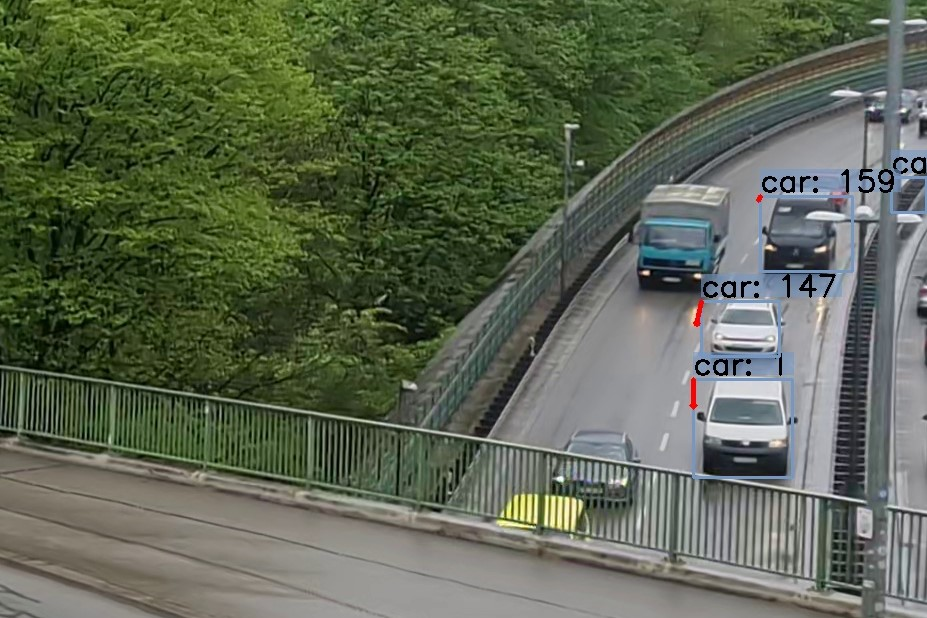
\includegraphics[width=7cm]{Media/LLost2.jpg}
			\caption{Keine Detektion des Fahrzeugs 61}
			\label{LLost2}
		\end{center}
	\end{figure}
	\begin{figure}[!h]
		\begin{center}
			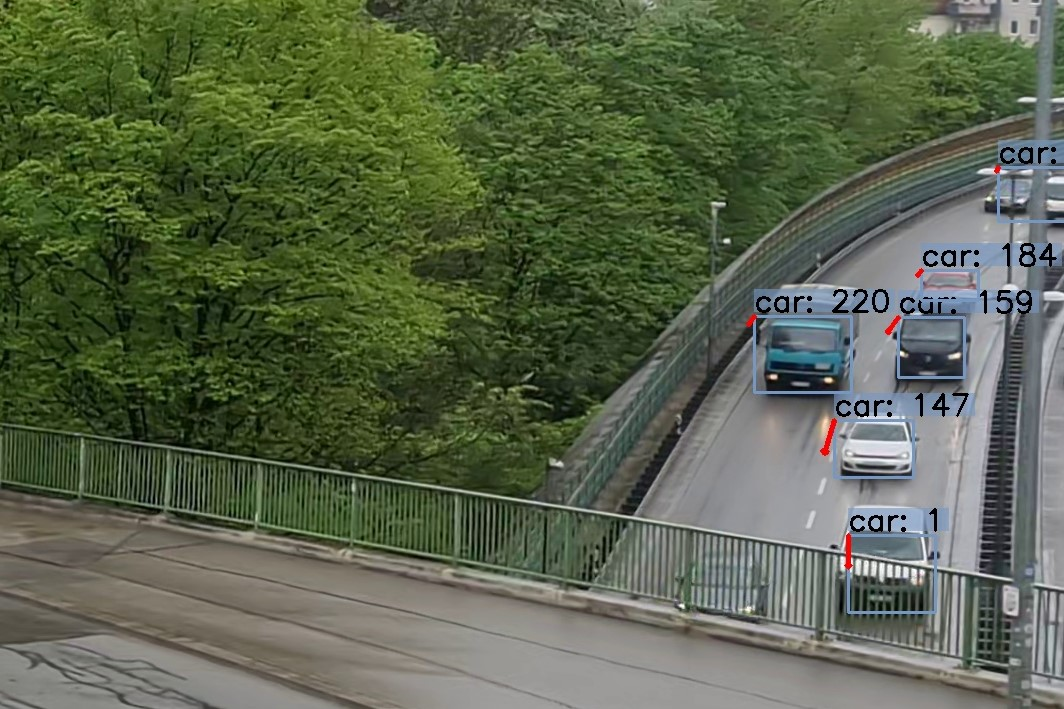
\includegraphics[width=7cm]{Media/LLost3.jpg}
			\caption{Neuzuweisung der ID}
			\label{LLost3}
		\end{center}
	\end{figure}
	
	Parameter die konfiguriert werden können sind die Zahl der Frames, ab wann der
	Track gelöscht wird. Zudem die Distanz zwischen einer Detektion und der von dem
	Kalman-Filter bestimmten Position. Zusätzlich kann der Wert der IoU-Distanz angegeben werden.
	Durch die Anpassung der maximalen IoU-Distanz
	kann ein häufiger Wechsel der ID mit direkt benachbarten Fahrzeugen vermieden werden.
	
	\subsubsection{Ergebnisse des Tracking mit SORT}
	Erneut basiert der Tracking-Algorithmus auf den Erkennungen des Objekt-Detektors. In Falle von SORT handelt es sich dabei um Gaussmixture. Dieser liefert teilweise für ein Objekt mehrere Erkennung. Dies liegt daran, dass Gaussmixture nicht das gesamte Objekt erkennt und die definierten Boundingboxen nicht das gesamte Objekt umschließen. SORT verarbeitet nur die erhaltenen Boundingboxen und kann daher nicht erkennen ob mehrere Boundingboxen zu einem Objekt gehören. Zu sehen ist die Problematik in Abbildung \ref{sortdouble}. Hierbei wurden zwei Boundingboxen für den Bus definiert. Ebenfalls zu erkennen ist, dass weder das gezeigte Auto, noch der Bus von einer Boundingbox einheitlich umschlossen sind. SORT kann allerdings die definierten Boxen korrekt verfolgen bis der Bus beziehungsweise das Auto den durch Gaussmixture abgedeckten Bereich verlässt. 
	
	\begin{figure}[!h]
		\begin{center}
			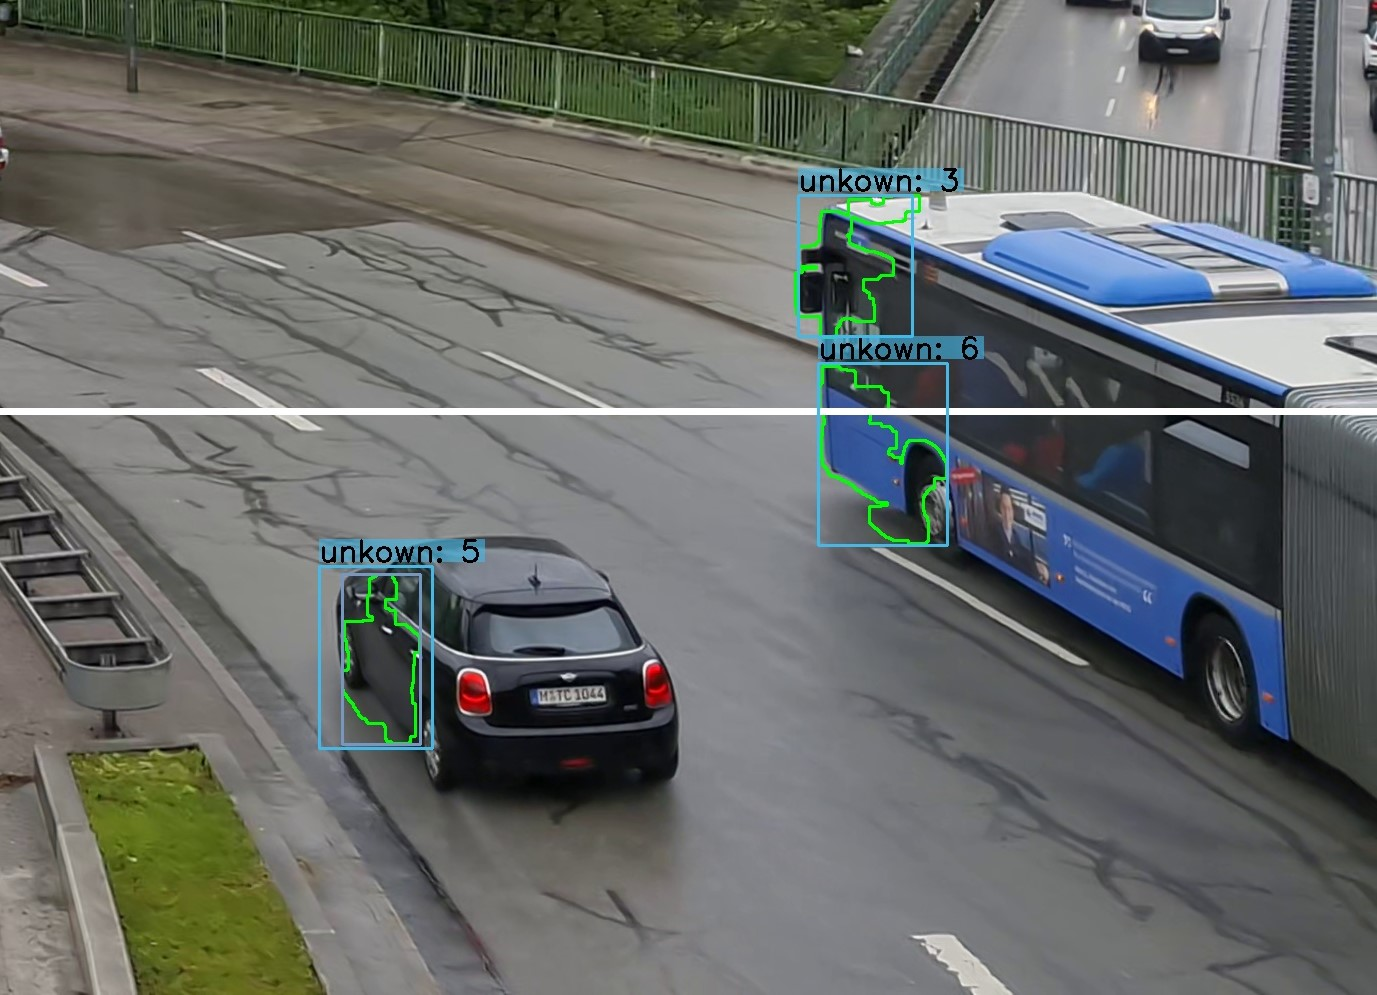
\includegraphics[width=7cm]{Media/sortdouble.jpg}
			\caption{Doppelte Erkennung eines Objekts. SORT unterscheidet nicht, daher zwei Tracking-IDs für den Bus}
			\label{sortdouble}
		\end{center}
	\end{figure}

	Da dieser Bereich sehr klein ist, ist auch die zurückgelegte Strecke der Fahrzeuge nicht ausreichend, um eine Aussage über das Tracking mit SORT über längere Distanz zu treffen. 
	
	
	\section{Zählen von Objekten}
	Wir testeten verschiedene Verfahren zu Zählen der gefundenen Objekte die das Video passieren.\\
	\textbf{Zählen der vergebenen TrackingID's.}\\
	 Unser erster Plan war das Zählen aller vergebenen Tracking ID's. Dies hätte den Vorteil, dass sobald ein Objekt gefunden wird auch gezählt wird. Wir stellten aber schnell fest, dass aufgrund von Fehlern in der Pipeline Objekten mehrfach neue IDs zugewiesen wurde. Diese Probleme entstehen in Kombination aus Fehlern in der Objekterkennung und dem Tracker. Je zuverlässiger das Tracking funktioniert desto geringer ist der Fehler im Zählen. Da aber ein perfekter Tracker nicht immer realistisch ist müssen bessere Lösungen gefunden werden.\\
	\textbf{Zähllinie.}\\
	 Um Trackingfehler zu umgehen wurde eine Zähllinie eingebaut, die sobald der Mittelpunkt der Boundingbox diese schneidet einmal hochzählt. Dies hatte noch immer Probleme wie zum Beispiel das manche Boxen doppelt gezählt wurden weil der Mittelpunkt kurz wieder nach oben rutschte. Manchmal wurde die Linie auch direkt übersprungen.\\
	\textbf{Zählung der Tracking IDs in einer Zählbox.}\\
	 Um die beiden Techniken zu vereinen wurde eine Zählbox entwickelt. So kann für jedes Szenario per Parameter die Position und Größe der Zählbox definiert werden. Sobald der Mittelpunkt einer Boundingbox in den die Zählbereich eindringt wird überprüft ob diese Tracking ID schon in einem Set enthalten ist. Ist sie es noch nicht wird hochgezählt. Es ist sinnvoll die Zählbox in Bereiche zu setzten in denen das Tracking zuverlässig funktioniert. 
	\begin{figure}[!h]
		\begin{center}
			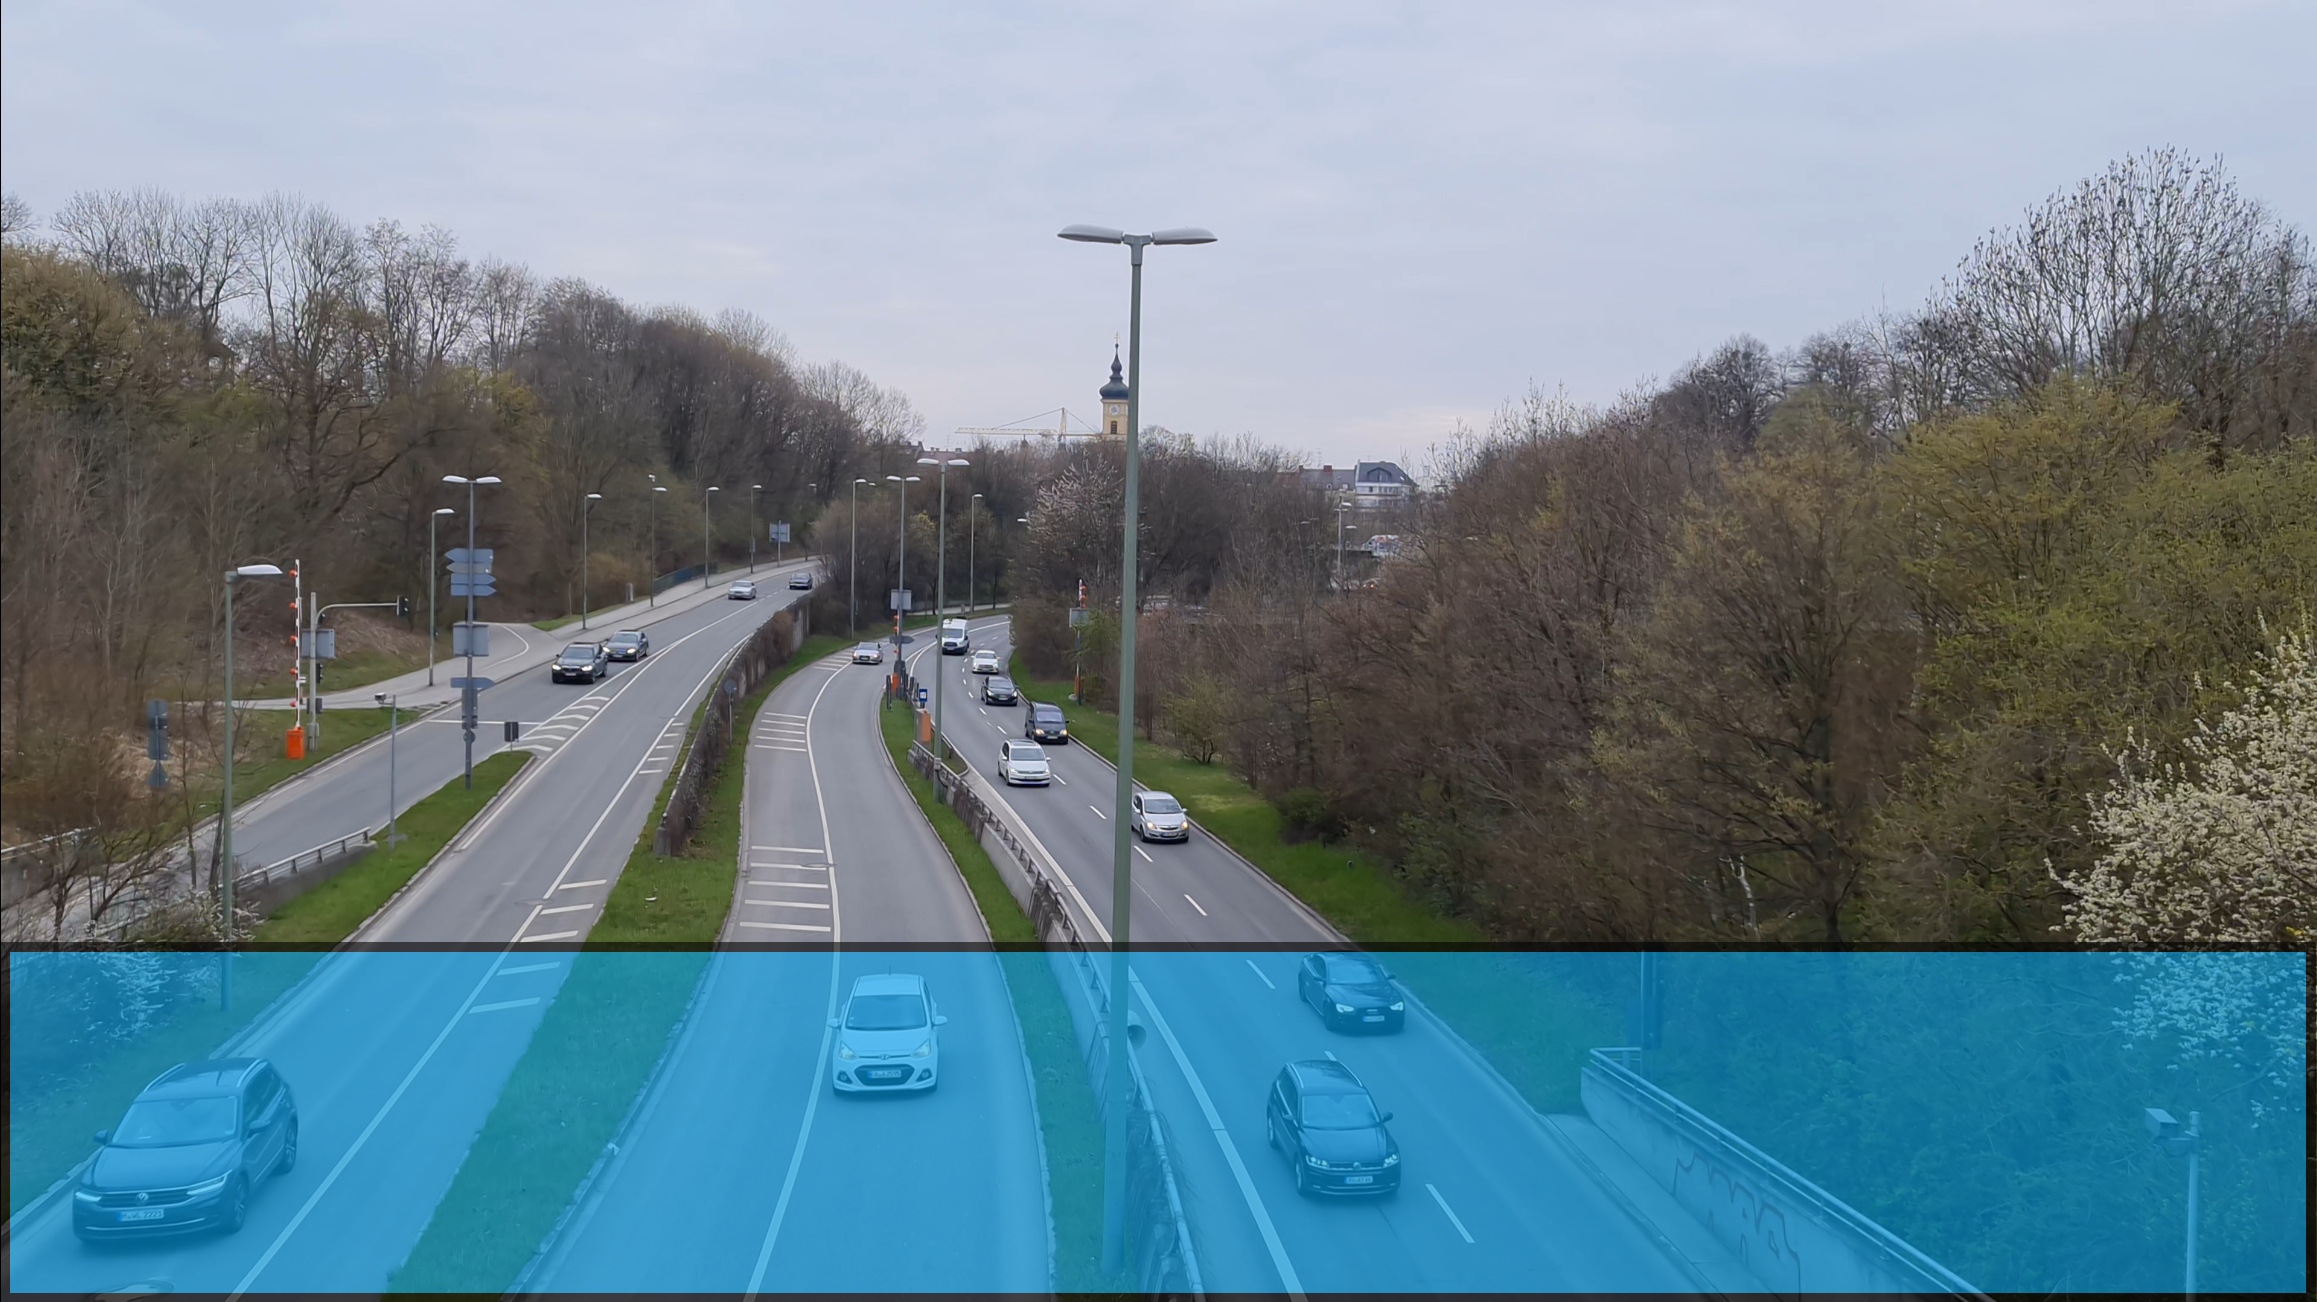
\includegraphics[width=7cm]{Media/BrudermuhlCounter.png}
			\caption{Darstellung einer Zählbox}
			\label{Counter}
		\end{center}
	\end{figure}
	
	\section{Zustandserkennung Züge}
	Da nun ein Objekt erfolgreich erkannt, verfolgt und seine Bewegungsrichtung erkannt werden kann, wird nun für Objekte die der Klasse Zug zugeordnet sind, die aktuelle Zugphase bestimmt.  
	Durch YOLO werden die Bounding Boxen pro Frame bestimmt. Durch Abgleich der TrackingID kann festgestellt werden, ob es sich immer um den selben Zug handelt. Für jede der Detektionen des ausgewählten Zugs wird durch Optical Flow die Magnitude und die Richtungswinkel bestimmt. Dabei wurde die durchschnittliche Richtung über die gesamten Richtungsvektoren der Bounding Box des Zuges bestimmt. Dies wurde im Verlauf des Projekts durch die Richtungsbestimmung des Kalmanfilters ersetzt, da diese zuverlässiger funktioniert. Dieser berechnet zusammen mit dem nächsten Zustand auch den Richtungsvektor, welcher genutzt wird. Fährt der Zug ein, hat dieses Objekt durch die Bewegung eine Magnitude größer 1. Der Richtungsvektor wird zur Visualisierung in das Bild als Pfeil eingefügt. Sobald der Zug erkannt wird und eine Richtung bestimmt wird, wechselt dessen Zustand von „Kein Zug“ zu „Einfahrend“. Dabei wird immer für 5 Frames geprüft ob die Richtung gleichbleibend ist. Sollte für eine Länge von 10 Frames die Magnitude unter 0 fallen ändert sich der Zustand des Zuges zu „Haltend“. Beginnt der Zug sich wieder zu bewegen und die Bewegung ist gleichbleibend in eine Richtung wird der Zustand auf „Abfahrend“ gesetzt, bis der Zug außerhalb des Bildes ist und nicht mehr erkannt wird.
	
	%TODO hier vielleicht Bild?
	
	\section{Vergleich klassischen Methoden mit Deep-Learning}
	Beide Verfahren haben ihre Stärken und Schwächen. Im Trackingteil sind beide Verfahren sich relativ ähnlich. Vor allem unterscheiden sich unsere Pipelines in der Objekterkennung welches dann aber auch maßgeblich die Trackingergebnisse beeinflusst. In der folgenden Liste werden die Vor- und Nachteile beider Verfahren nach unserer Erkenntnissen aufgeschlüsselt.
	\begin{enumerate}
		\item \textbf{Genauigkeit:} Die Deep-Learning Verfahren verzeichnen vor allem gute Out-Of-The-Box Leistung. Ohne große Hyperparameteroptimierung erreicht man schnell eine ausgezeichnete Performance. Klassische Verfahren können dabei auch sehr gute Leistung erzielen wenn genug Optimierung stattfindet. Der Aufwand der Optimierung ist aber stark von der Situation abhängig.\\
		So stellten wir fest das die klassischen Verfahren deutlich fehleranfälliger bei schlechten Videoaufnahmen waren. Verwackelte Aufnahmen stellten eine große Herausforderung dar. Gegenmaßnahmen dafür sind ein Stativ oder andere auf Software basierende Verfahren. Die Objekterkennung basierend auf YoloV4 hat überhaupt kein Problem mit verwackelten Bildern da es jeden Frame unabhängig von einander betrachtet. Die Tracking-Algorithmen sind bezüglich starker Bewegung jedoch anfällig, da die Vorhersage der nächsten Position und der Assoziation der Detektion erschwert wird. DeepSort nutzt für die Assoziation bei starker Bewegung daher hauptsächlich den Feature-Vektor um die Objekte zuzuordnen. Es lässt sich sagen das die meisten Fehler der Tracker auf schlechter Objekterkennung basieren. DeepSORT ist dabei etwas weniger fehleranfällig als SORT.
		
		\item \textbf{Laufzeit:} Bei der Laufzeit haben die klassischen Verfahren einen klaren Vorteil. Hier erzielten wir etwa doppelt so viele Bilder pro Sekunde als bei den DeepLearning Methoden. Außerdem dürfte es schwieriger sein Deep-Learning Verfahren auf Embedded Geräten lauffähig zu bekommen. Prinzipiell sollten beide Methoden auf Grafikkarten beschleunigt werden können.
		
		\item \textbf{Nachvollziehbarkeit:} Bei Fehlern in der Objekterkennung bei Yolo ist es häufig schwierig nachzuvollziehen wie diese entstanden. Auch ist das behandeln dieser Fehler schwieriger. Bei MOG ist dies deutlich einfacher, da man nur das Graubild untersuchen muss und dann die Hyperparameter anpassen muss.
		
		\item \textbf{Implementierungsaufwand:} Es kann gesagt werden das die Implementierung der klassischen Verfahren deutlich einfacher ist wie die der DeepLearning Methoden. Außerdem muss beachtet werden das ein trainiertes Netz vorhanden sein muss. Ist dieses nicht vorhanden muss erst ein Datensatz aufwendig erstellt werden mit welchen dann ein Netz trainiert werden muss.
		
	\end{enumerate}
	Zusammenfassend lässt sich sagen das beide Verfahren ihre Stärken haben. Die Entscheidung welche Methode verwendet werden sollte hängt stark von der Situation und den verfügbaren Ressourcen ab.
	
	\begin{thebibliography}{00}
		\bibitem{z1}https://www.zeit.de/news/2020-10/18/s-bahn-stammstrecke-in-muenchen-fuer-arbeiten-gesperrt
		\bibitem{mog1}http://www1.ece.neu.edu/~schirner/cv/AsilomarSCC13\_MoG.pdf
		\bibitem{stab}https://de.wikipedia.org/wiki/Bildstabilisierung
		\bibitem{s1}https://learnopencv.com/video-stabilization-using-point-feature-matching-in-opencv/
		\bibitem{s2}https://docs.opencv.org/3.4/d4/dee/tutorial\_optical\_flow.html
		\bibitem{s3}https://docs.opencv.org/3.4/d4/d8c/tutorial\_py\_shi\_tomasi.html
		\bibitem{s4}https://docs.opencv.org/3.4/dc/d6b/group\_\_video\_\_track.html
		\bibitem{ed}https://docs.opencv.org/3.4.12/db/df6/tutorial\_erosion\_dilatation.html
		\bibitem{m1}https://www.cs.hs-rm.de/~ulges/teaching/15MLSEM/files/folien/suhr.pdf
		\bibitem{m2}https://opencv24-python-tutorials.readthedocs.io/en/latest/py\_tutorials/py\_video/py\_bg\_subtraction/py\_bg\_subtraction.html
		\bibitem{m3}https://link.springer.com/article/10.1007/s10462-017-9542-x
		\bibitem{m4}https://docs.opencv.org/3.4/d1/dc5/tutorial\_background\_subtraction.html
		
		\bibitem{b0}https://medium.com/@sarangzambare/object-detection-using-non-max-supression-over-yolov2-382a90212b51
		\bibitem{b1}https://arxiv.org/pdf/1506.02640v5.pdf
		\bibitem{b2}https://arxiv.org/pdf/2004.10934.pdf %V4
		\bibitem{b3}https://arxiv.org/pdf/1612.08242.pdf %V2
		\bibitem{b4}https://pjreddie.com/media/files/papers/YOLOv3.pdf %V3
		\bibitem{b5}https://jonathan-hui.medium.com/real-time-object-detection-with-yolo-yolov2-28b1b93e2088 % V1 Loss
		\bibitem{b6}https://openaccess.thecvf.com/content\_cvpr\_2017/papers/Lin\_Feature\_Pyramid\_Networks\_CVPR\_2017\_paper.pdf % FPN
		\bibitem{b7}https://arxiv.org/vc/arxiv/papers/1908/1908.08681v1.pdf%MISH
		\bibitem{b8}https://jonathan-hui.medium.com/yolov4-c9901eaa8e61 %Yolov4 Hui
		\bibitem{b9}https://arxiv.org/pdf/1406.4729.pdf %SPP
		\bibitem{b10}https://arxiv.org/pdf/1803.01534.pdf %PAN
	\end{thebibliography}
	
	\section{Anhang}
	
	
\end{document}
